% TODO: stichpunkte als fließtext soweit möglich (reflexion & fazit). vielleicht auch in anderen abschnitten (kapitel 2, ab seite 10).

\subsection{Prompt-Setup: Einheitliche Aufgabenstellung für alle Tools}
\label{sec:prompt-setup}

Um eine objektive und vergleichbare Bewertung zu ermöglichen, wurde für die
Implementierung des Map-Screens in allen drei Tools (\textit{GitHub Copilot},
\textit{Cursor}, \textit{Bolt.new}) derselbe, detaillierte Prompt verwendet,
der die funktionalen und technischen Anforderungen klar definierte:

\begin{lstlisting}[]
    Create a Map Screen with Event Markers and Filter in React Native
    
    Create a React Native component called `MapScreen` that displays event markers on a map using event data from the `EventsProvider` context.
    
    ## Requirements
    
    ### Functionality
    - Use the list of events from the `EventsProvider` context.  
      (Access: `const { events, loading, error, refreshEvents } = useEvents();`)
    - Each event contains:
      - `docId: string`
      - `title: string`
      - `category: string`
      - `date: string`
      - `geoPoint: { latitude: number; longitude: number }`
    - Example Context Usage: const { events, loading, error, refreshEvents } = useEvents();
    - Display all events as markers on a map (`react-native-maps` or Expo MapView).
    - When a marker is tapped, show a callout or modal with event details (`title`, `time`, `category`, optional image/avatar).
    - Add filter options above the map (e.g. by category, date, distance).  
      Only display events that match active filters.
    - Handle loading and error states appropriately.
    
    ### UI/UX
    - Modern mobile UI with a clean filter bar on top, responsive marker popups, and a loading spinner.
    - Use functional components and React hooks (TypeScript).
    - Styling should be clean and minimal (simple css with StyleSheet prefered).
    - Map should fit all visible markers and allow user zoom/pan.
    - Compatible with Expo.
    
    ### File Structure
    - Main screen in `map.tsx`.
    - Optional: Reusable `EventMarker` component.
    
    ### Additional
    - Keep code modular, clean, and well-commented.
    - Focus on maintainability and clarity.
    - Use the attached layout (filter bar on top, map below, details as bottom sheet/callout) as a visual reference.
    
    ### Example Event Type (TypeScript)
    interface Event {
      docId: string;
      title: string;
      category: string;
      date: string;
      geoPoint: { latitude: number; longitude: number };
      // ...more fields possible
    }

    ## Goal
    A fully functional, modern React Native map screen with event markers, filter bar, marker popups, and proper handling of loading/error states -- ready to integrate into an Expo app.

    
    \end{lstlisting}

\noindent
\textbf{Hinweis:} Diese Aufgabenstellung wurde in allen Demonstrationen identisch genutzt, um die Unterschiede in Lösungsstrategie und Codequalität der Tools direkt vergleichbar zu machen.

\subsection{Demonstration mit GitHub Copilot}

\subsubsection{Setup und Vorgehen}
Die Entwicklung des Map-Screens wurde exemplarisch mit \textbf{GitHub Copilot}
in Visual Studio Code durchgeführt. Für größtmögliche Vergleichbarkeit kamen
ausschließlich die Copilot-Funktionen zum Einsatz, keine weiteren KI-Plugins.

\begin{figure}[htbp]
      \centering
      \vspace{1em}
      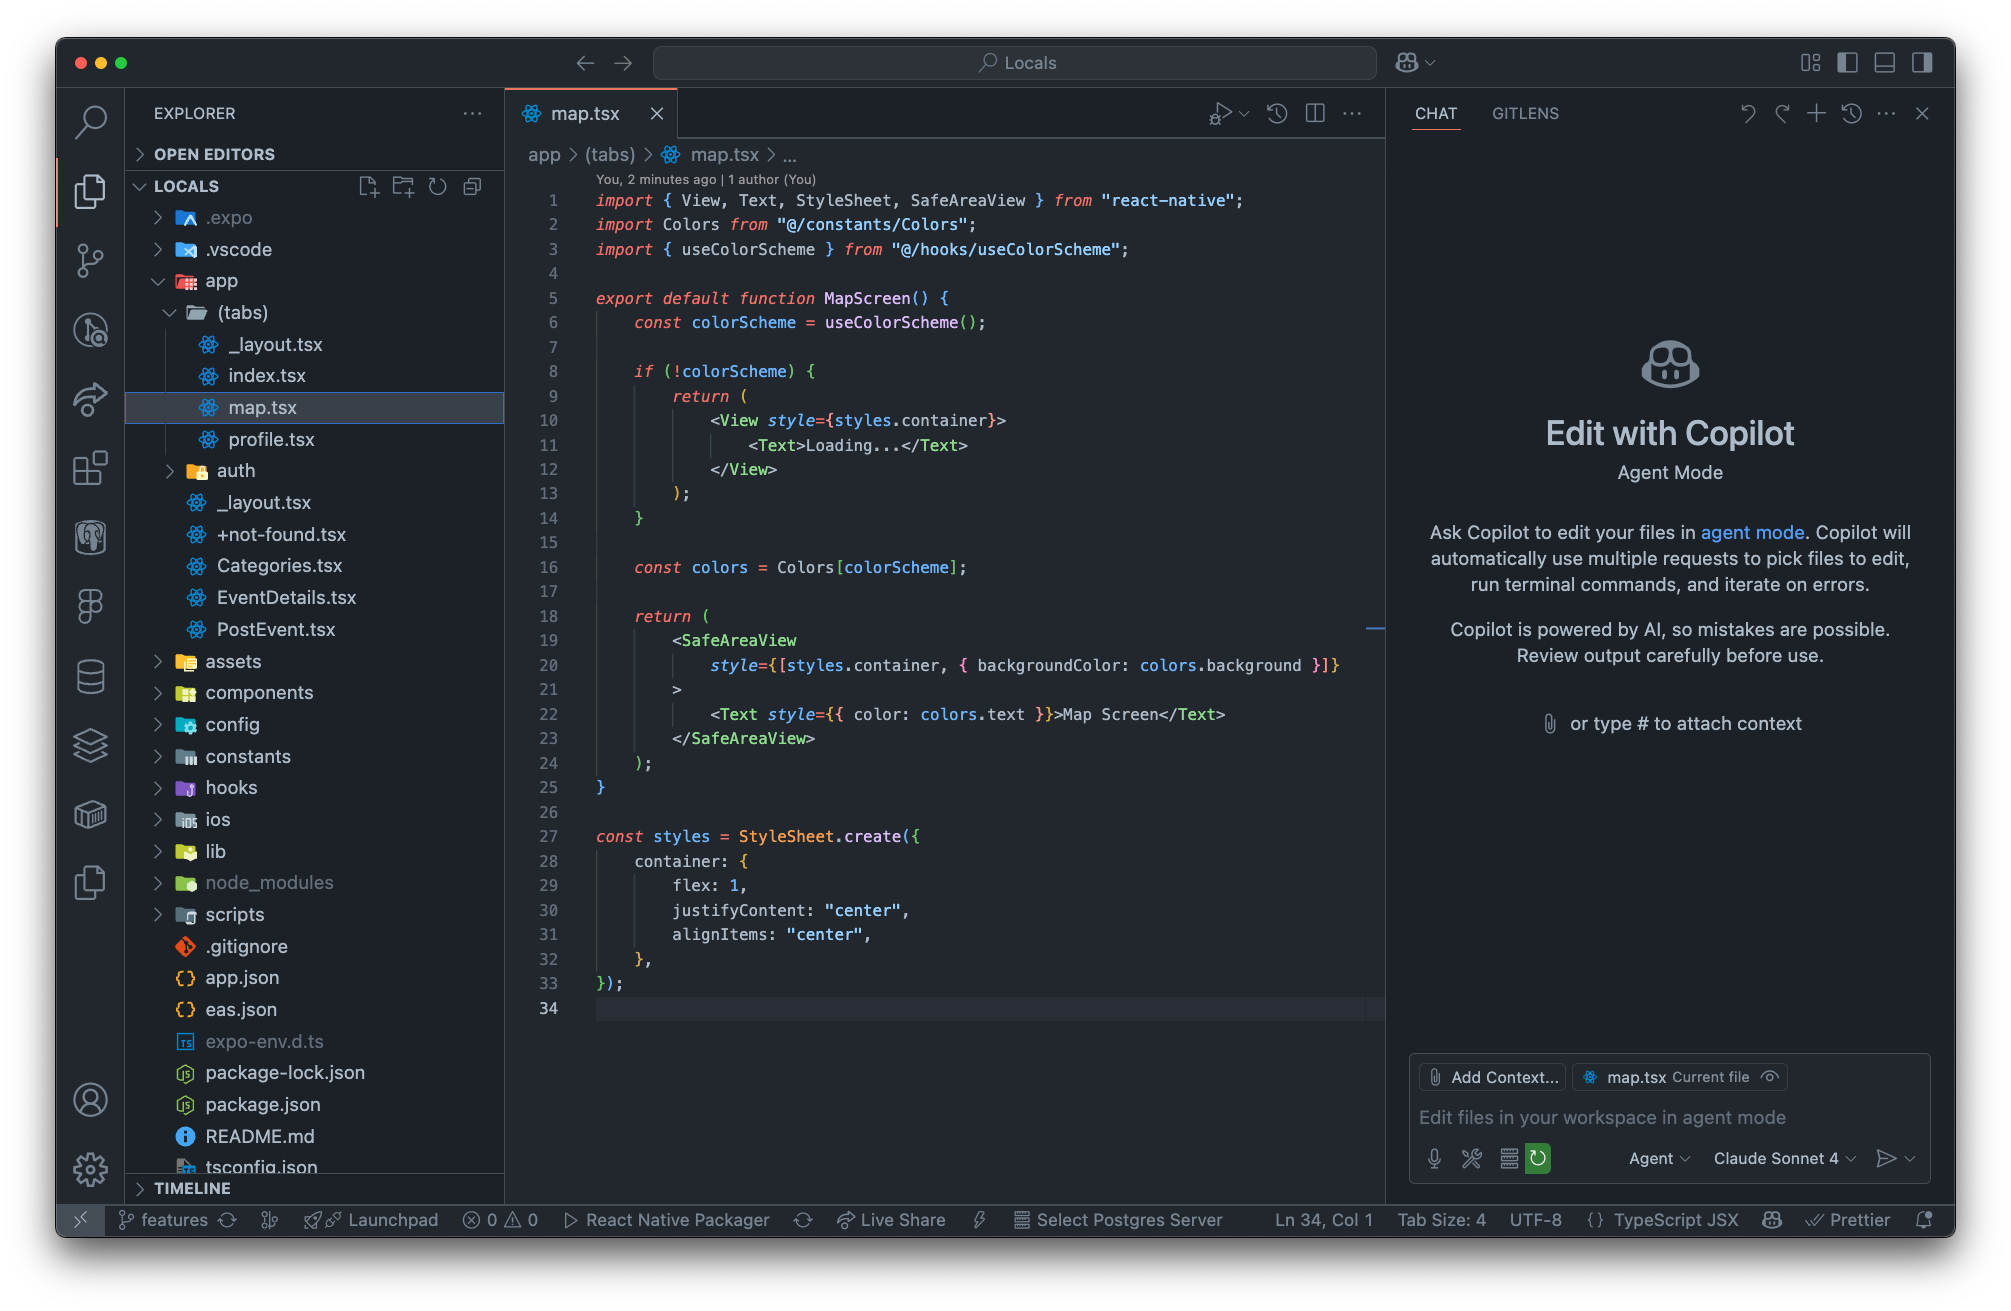
\includegraphics[width=1\textwidth]{images/copilot_screenshots/Screenshots Ist-Zustand-copilot.png}
      \caption{Ausgangszustand der Anwendung vor dem Einsatz von Copilot. \textit{Copilot-Demo}}
      \label{fig:copilot-istzustand}
\end{figure}

% TODO: muss ich alles aufzählen nicht nur z.b.?
Zu Beginn wurde die Entwicklungsumgebung vorbereitet (z.~B.\ Installation von
\texttt{react-native-maps} und \texttt{expo-location}). Die Aufgabenstellung
wurde als Kommentar oder Docstring auf Englisch eingefügt (\emph{siehe
      Abschnitt~\ref{sec:prompt-setup}}).

\subsubsection{Schrittweise Umsetzung und Reflexion}
Die Entwicklung erfolgte nach folgendem Muster:
\begin{enumerate}
      \item \textbf{Prompt definieren:} Pro Feature (z.\,B. Marker, Filter, Event-Details) wurde ein spezifischer Kommentar als Arbeitsanweisung eingefügt.
      \item \textbf{Vorschläge von Copilot akzeptieren oder anpassen:} Vorschläge wurden übernommen, angepasst oder verworfen.
      \item \textbf{Test und Dokumentation:} Nach jeder Änderung wurde der Code getestet und die Funktionsweise reflektiert.
      \item \textbf{Fehlersuche und Nacharbeit:} Fehlerhafte Vorschläge oder Bugs wurden durch Rücksprache mit Copilot, Recherche oder manuelle Nacharbeit behoben.
\end{enumerate}

\begin{figure}[htbp]
      \centering
      \vspace{1em}
      \begin{minipage}{0.48\textwidth}
            \centering
            \includegraphics[width=0.98\textwidth]{images/copilot_screenshots/implementation-rückmeldung-copilot-1.png}
      \end{minipage}
      \hfill
      \begin{minipage}{0.48\textwidth}
            \centering
            \includegraphics[width=0.98\textwidth]{images/copilot_screenshots/implementation-rückmeldung-copilot-2.png}
      \end{minipage}
      \caption{Rückmeldung und Hinweise von Copilot während der Implementierung. \textit{Copilot-Demo}}
      \label{fig:copilot-impl-pair}
\end{figure}

\noindent Die technische Umsetzung umfasste:
\begin{itemize}
      \item Anzeige aller Events als Marker (mit Kategorie und Titel) auf der Karte.
      \item Filterleiste zur Auswahl nach Kategorie und Datum.
      \item Darstellung von Event-Details beim Tippen auf einen Marker.
      \item Responsives Layout, modernes UI-Design, Fehler- und Ladezustände.
\end{itemize}

\begin{figure}[htbp]
      \centering
      \vspace{1em}
      \begin{minipage}{0.48\textwidth}
            \centering
            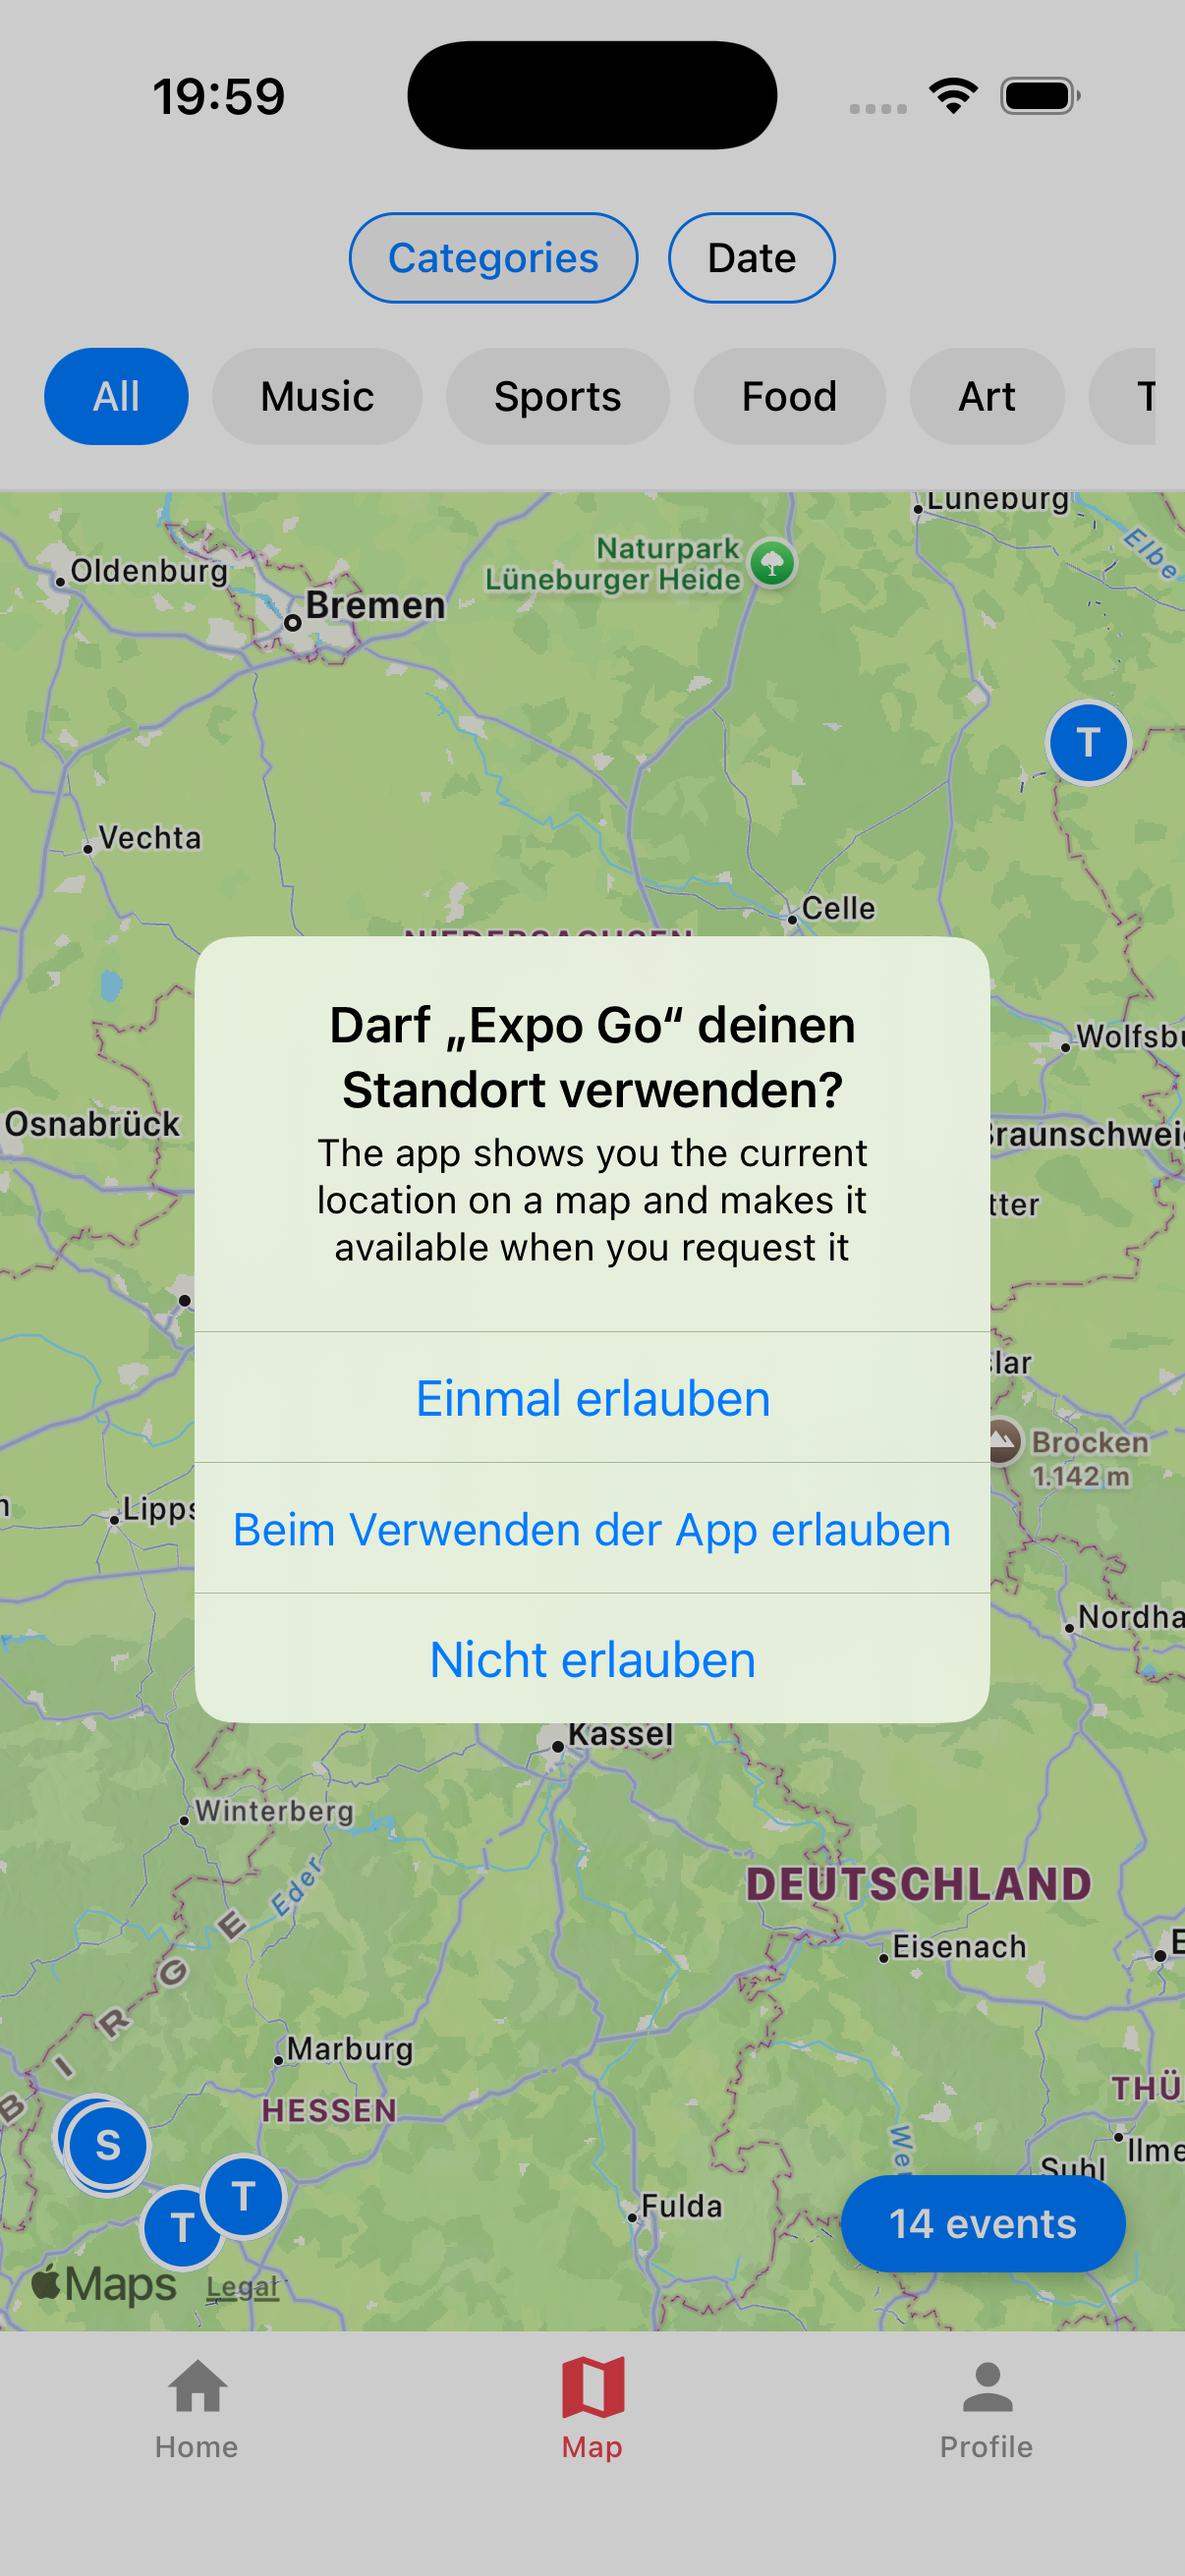
\includegraphics[width=\textwidth]{images/copilot_screenshots/6. 1. Version das MapScreens - Screenshot-copilot.png}
            \caption{Erste lauffähige Version des MapScreens nach KI-gestützter Entwicklung. \textit{Copilot-Demo}}
      \end{minipage}
      \hfill
      \begin{minipage}{0.48\textwidth}
            \centering
            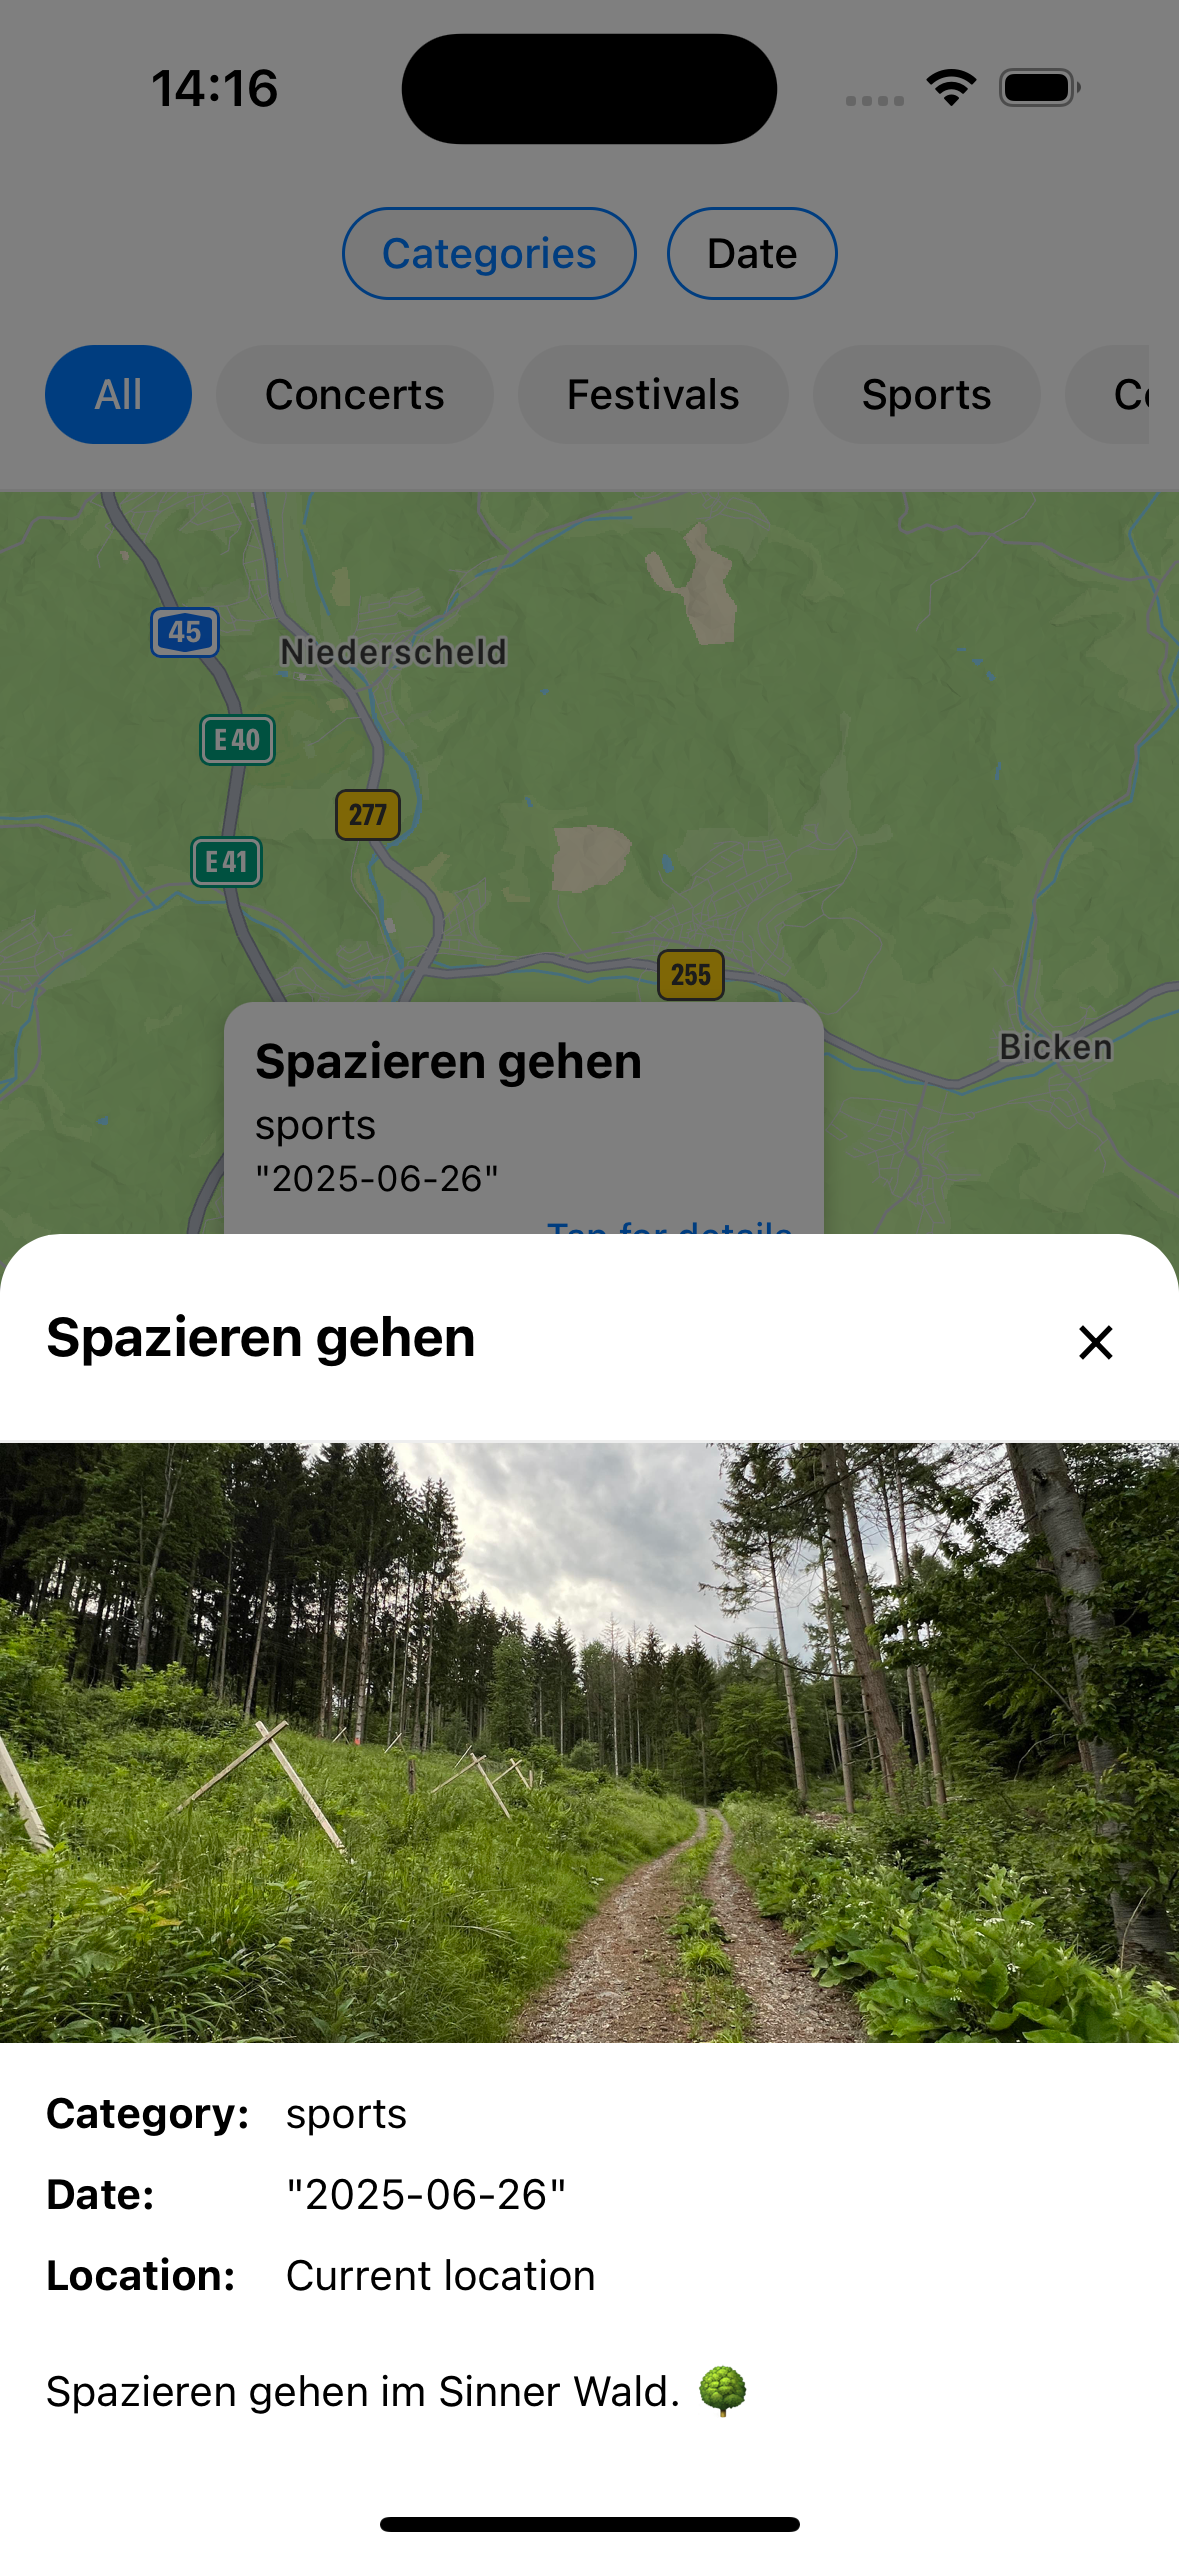
\includegraphics[width=\textwidth]{images/copilot_screenshots/Callouts+modal-copilot.png}
            \caption{Event-Details und Callouts auf dem MapScreen. \textit{Copilot-Demo}}
            \label{fig:copilot-callouts}
      \end{minipage}
\end{figure}

% TODO: "..und meist nachvollziehbar" -> was lief denn nicht nachvollziehbar? was will ich damit sagen? hier zb. immer punkt 
Die Code-Generierung erfolgte modular und meist nachvollziehbar. Copilot
erstellte automatisch das Grundgerüst der Map-Komponente und ergänzte Schritt
für Schritt die Logik für Marker, Filter und Event-Details.

\textbf{Stärken:}
\begin{itemize}
      \item Effiziente Generierung von Boilerplate-Code und wiederkehrenden Patterns.
      \item Schnelle Vorschläge für UI-Komponenten und Interaktionslogik.
      \item Erkennung von einfachen Fehlern und automatische Typanpassung.
\end{itemize}

\textbf{Schwächen und typische Fehlerquellen:}
\begin{itemize}
      \item Teilweise fehlerhafte oder veraltete Import-Pfade.
      \item Missverständnisse bei nicht exakt spezifizierten Datenstrukturen.
      \item Filter-Logik für den ``All''-Filter funktionierte zunächst nicht wie erwartet.
      \item Bei komplexeren Anforderungen blieb Nacharbeit notwendig.
\end{itemize}

\textbf{Reflexion:}
\begin{itemize}
      \item Die Vorschläge waren bei Standardaufgaben meist brauchbar (subjektive
            Zufriedenheit: 4/5), bei komplexeren State- oder Typ-Logiken oft unvollständig.
      \item Die Interaktion mit Copilot war intuitiv, erfordert aber genaue Prompts und ein
            grundsätzliches Verständnis für Implementierungsdetails.
      \item Bei UI-Details oder individuellen Anforderungen blieb Nacharbeit unerlässlich.
\end{itemize}

\textbf{Fazit:}
Copilot ist ein leistungsfähiges Assistenz-Tool, das Routinearbeiten erheblich beschleunigt. Bei komplexeren Anforderungen stößt es jedoch an Grenzen, sodass eine kritische Prüfung und manuelle Nacharbeit unverzichtbar bleiben. Die Demonstration belegt, dass Copilot einen relevanten Effizienzgewinn für erfahrene Entwickler:innen bieten kann, den Anspruch auf vollständige Automatisierung jedoch noch nicht erfüllt.

\subsection{Demonstration mit Cursor}

% TODO: Cursor hier fett geschrieben, sonst kursiv. einheitlich schreiben.
\subsubsection{Setup und Vorgehen}
Für die Entwicklung des Map-Screens wurde \textbf{Cursor} als spezialisierte
KI-basierte Entwicklungsumgebung genutzt (Branch: \texttt{cursor},
Sprachmodell: Claude 3.7 Sonnet, Agent mode). Auch hier wurde die identische
Aufgabenstellung genutzt (\emph{siehe Abschnitt~\ref{sec:prompt-setup}}).

\begin{figure}[htbp]
      \centering
      \vspace{1em}
      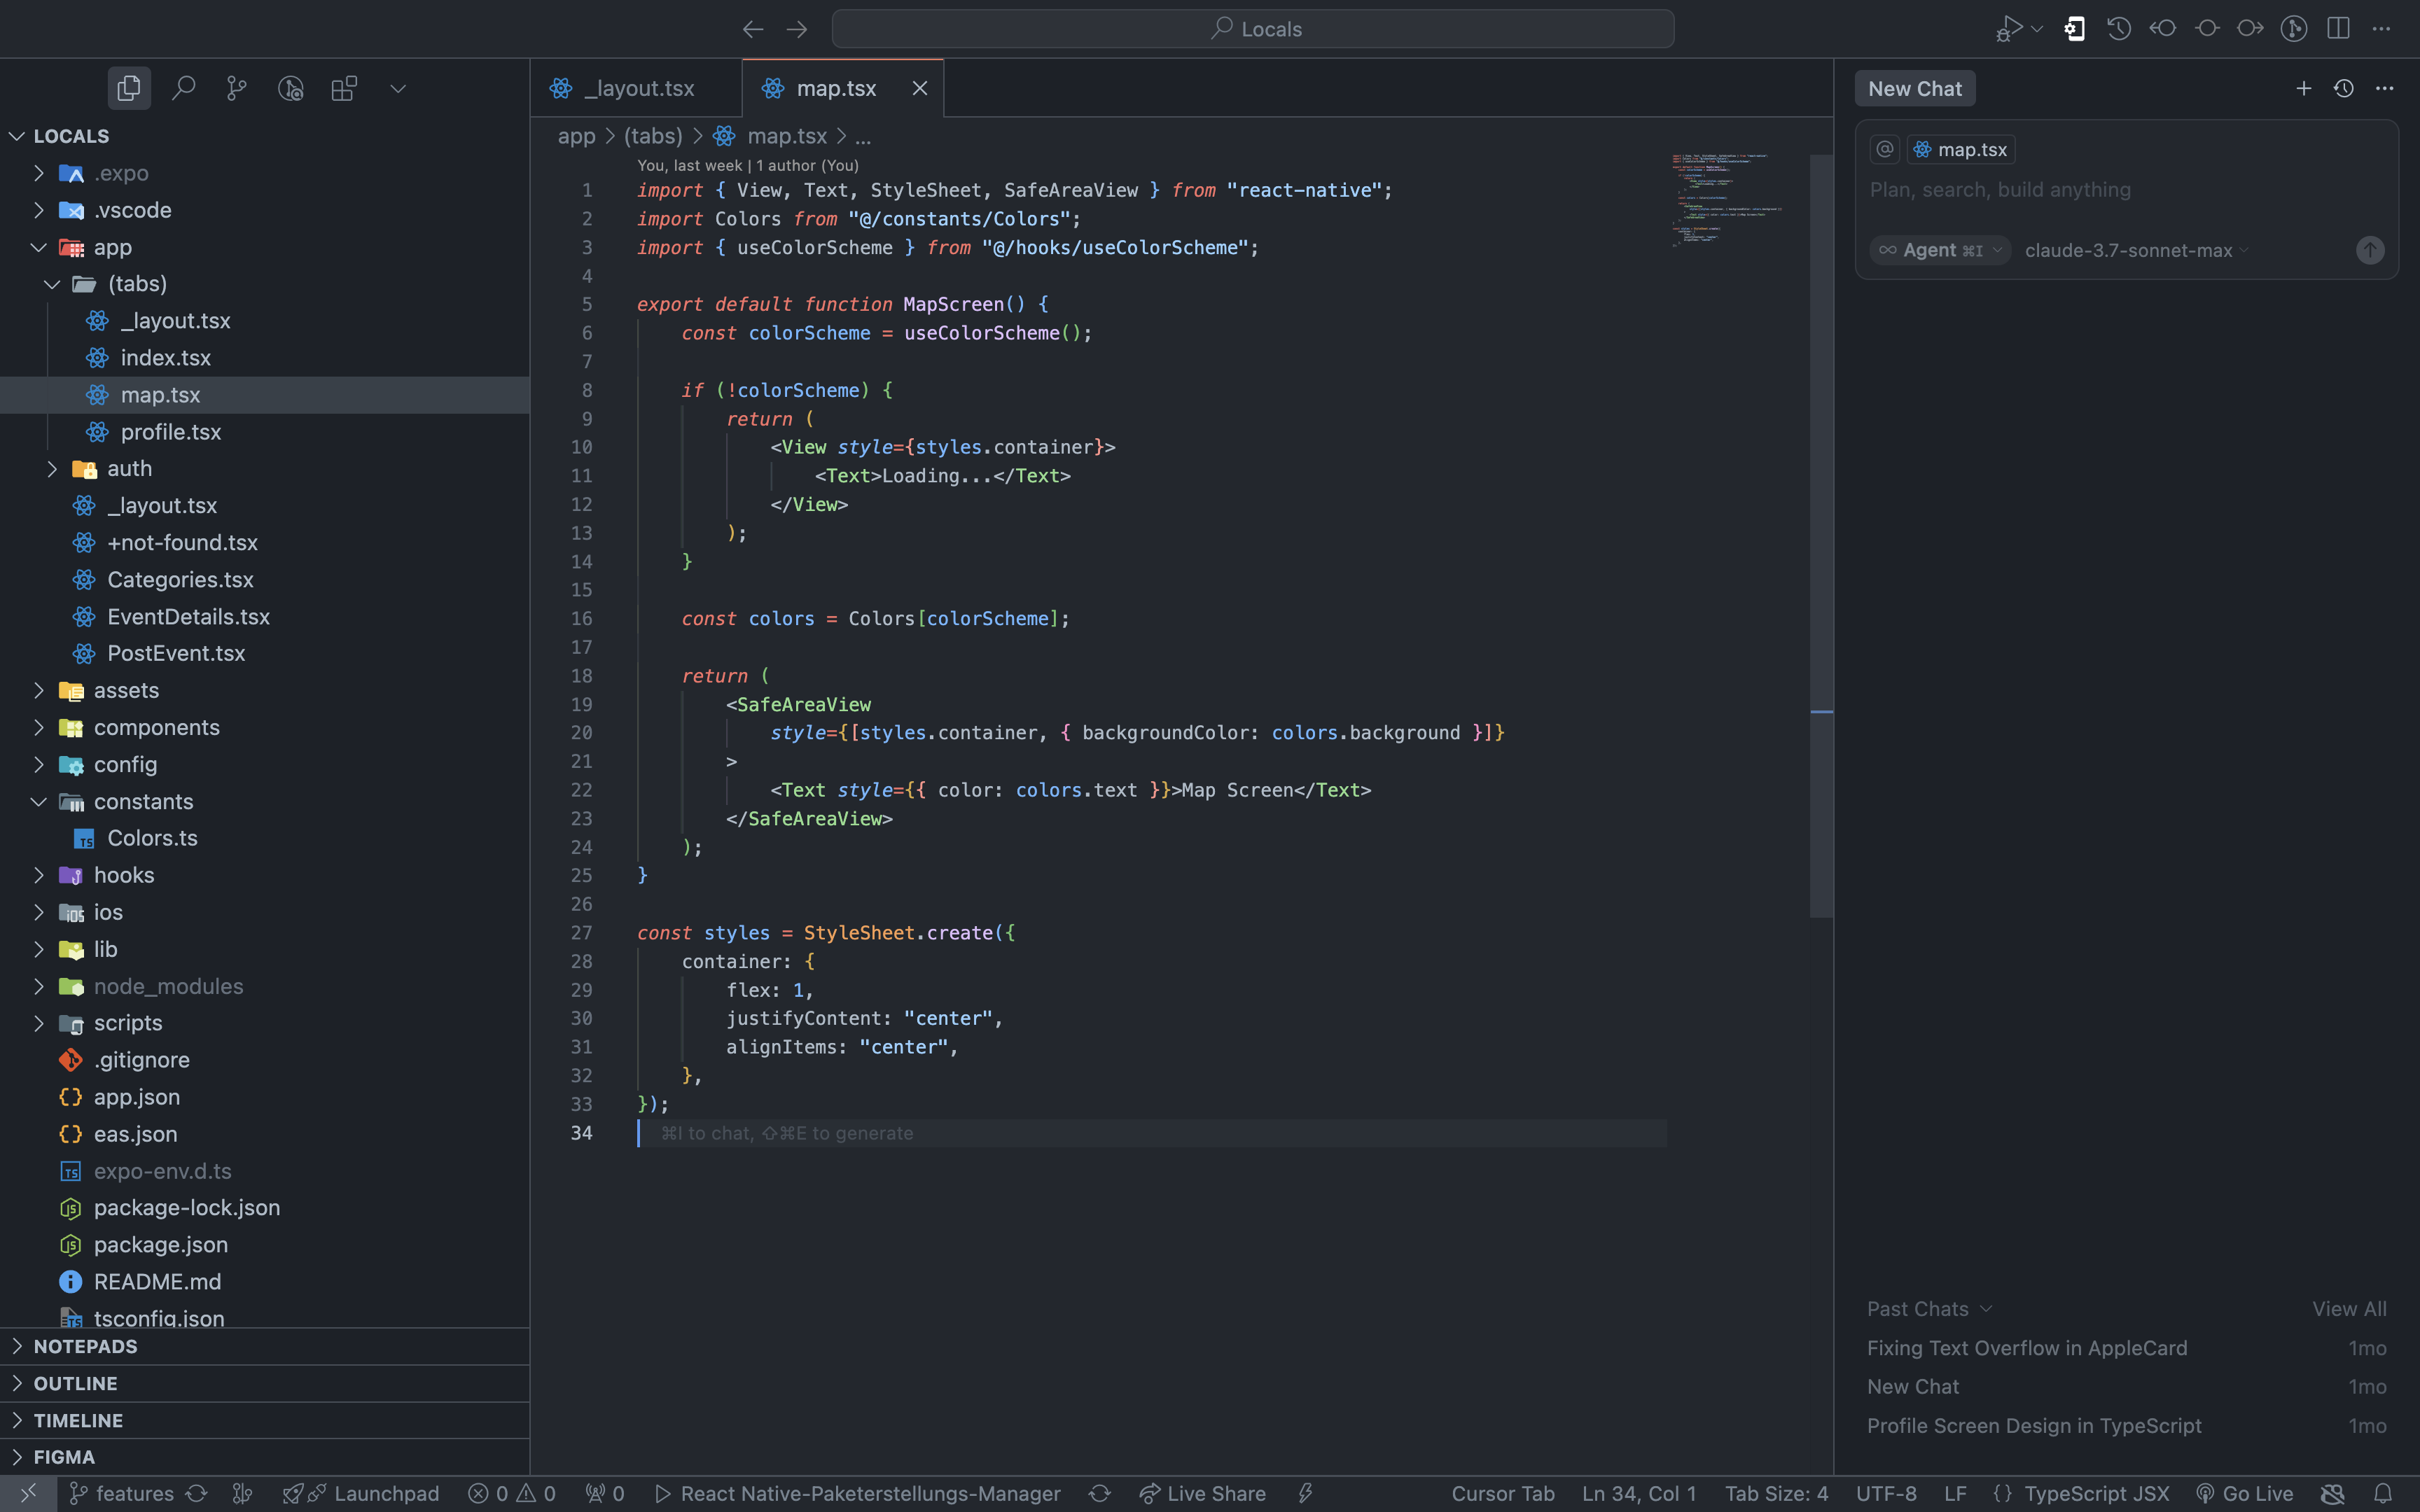
\includegraphics[width=1\textwidth]{images/cursor_screenshots/Screenshots Ist-Zustand-cursor.png}
      \caption{Ausgangszustand der Anwendung vor Einsatz von Cursor. \textit{Cursor Demo}}
      \label{fig:cursor-istzustand}
\end{figure}

Zu Beginn wurden Screenshots des aktuellen App-Zustands sowie relevanter
Komponenten (u.\,a. \texttt{\_layout.tsx}, Event Provider) als Kontext
bereitgestellt.

\subsubsection{Schrittweise Umsetzung und Reflexion}

Der Entwicklungsprozess war durch mehrere Besonderheiten gekennzeichnet:

\begin{enumerate}
      \item \textbf{Prompt Chaining und Screenshot-Kontext:} Zu jedem Entwicklungsschritt wurden gezielt neue Prompts mit aktualisierten Anforderungen und Referenz-Screenshots gestellt.
      \item \textbf{Terminal-Steuerung:} Cursor führte notwendige Terminalbefehle (z.\,B. Paketinstallationen) eigenständig aus und dokumentierte Fehlermeldungen sowie Lösungsvorschläge direkt im Chat.
      \item \textbf{Debugging und Package-Kompatibilität:} Cursor identifizierte eigenständig Kompatibilitätsprobleme, z.\,B. bei der \texttt{react-native-maps}-Version, und schlug proaktiv eine Anpassung auf die funktionierende Version vor.
\end{enumerate}

\begin{figure}[htbp]
      \centering
      \vspace{1em}
      \begin{minipage}{0.48\textwidth}
            \centering
            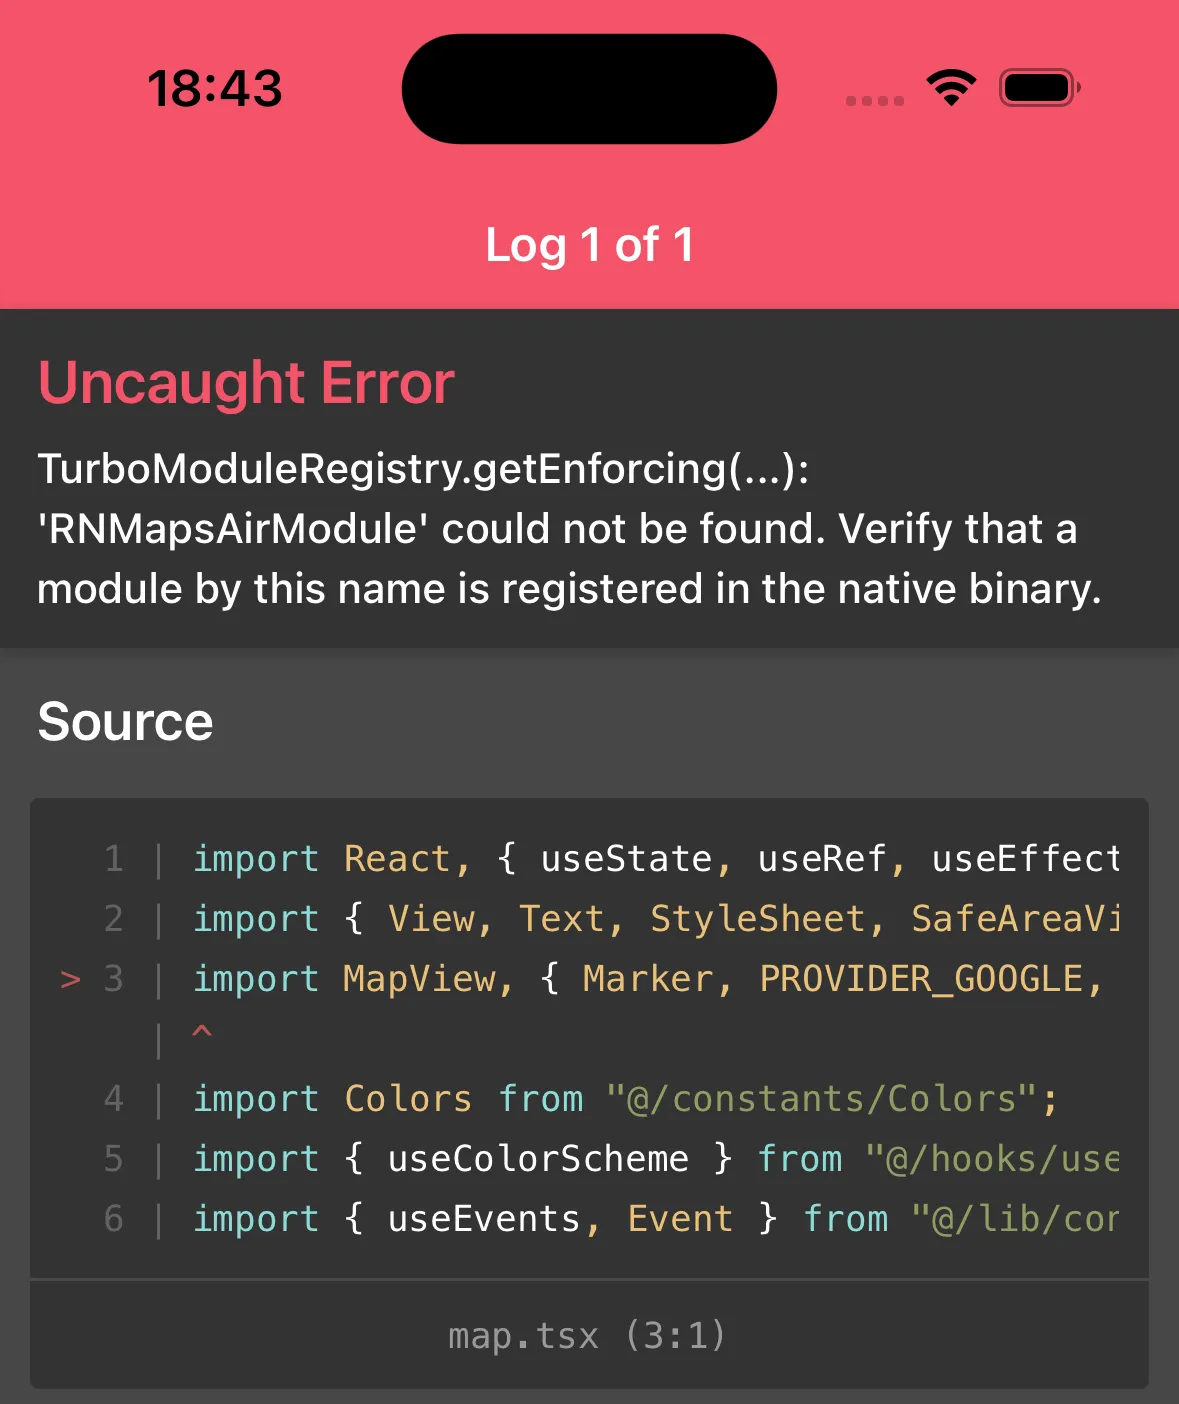
\includegraphics[width=0.98\textwidth]{images/cursor_screenshots/(NOBRIDGE) ERROR-cursor.png}
      \end{minipage}
      \hfill
      \begin{minipage}{0.48\textwidth}
            \centering
            \includegraphics[width=0.98\textwidth]{images/cursor_screenshots/Cursor führt terminal befehle eigenständig aus.png}
      \end{minipage}
      \caption{Typische Fehlermeldung und autonomes Ausführen von Terminalbefehlen durch Cursor beim Einrichten des MapScreens. \textit{Cursor-Demo}}
      \label{fig:cursor-error-terminal}
\end{figure}

\begin{enumerate}[resume]
      \item \textbf{Iterative Korrekturen und UX-Verbesserungen:} Bei UI-Problemen (z.\,B. überlagernde Filter/Buttons) wurden nach Rückmeldung gezielt Layout-Vorschläge unterbreitet.
      \item \textbf{Feature-Integration:} Funktionen wie Filter, Refresh-Button und Navigation zu Event-Standorten wurden auf Nachfrage oder eigenständig ergänzt.
\end{enumerate}

\begin{figure}[htbp]
      \centering
      \vspace{1em}
      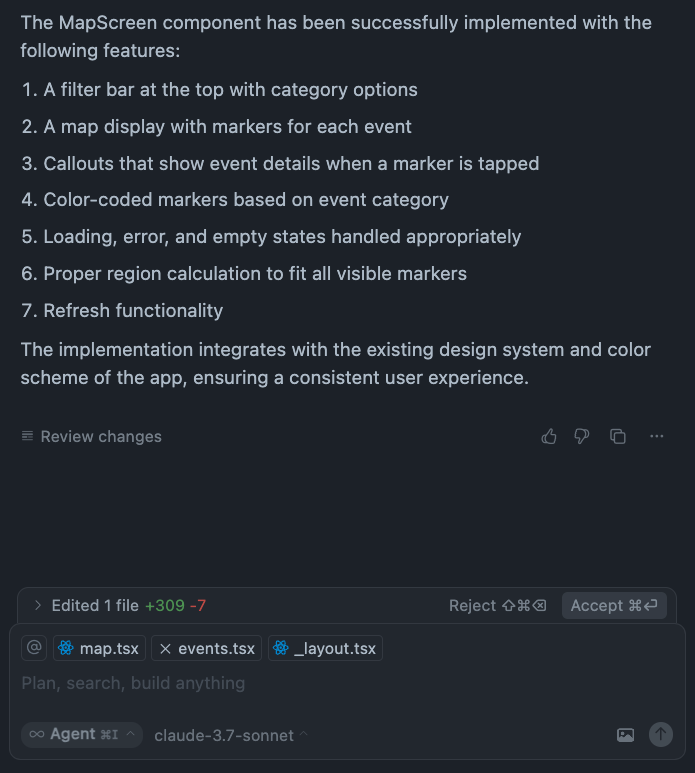
\includegraphics[width=0.48\textwidth]{images/cursor_screenshots/erster durchgang-cursor.png}
      \caption{Erste Umsetzungsschritte nach Bereitstellung des Kontexts und initialem Prompt. \textit{Cursor-Demo}}
      \label{fig:cursor-erster-durchgang}
\end{figure}

\textbf{Besonders positiv fiel auf:}
\begin{itemize}
      \item Cursor war bei der Behebung von Package-Fehlern und bei der automatischen
            Adaption von Code an neue Datenstrukturen sehr präzise.
      \item Im Vergleich zu Copilot wurde die grundlegende Kartenfunktion schneller
            funktionsfähig, auch wenn die erste Map-Anzeige erst nach mehreren Prompts
            erschien.
      \item Cursor dokumentierte seine Debugging-Schritte transparent und schlug auch
            Lösungen für übersehene Fehlerquellen vor.
\end{itemize}

\begin{figure}[htbp]
      \centering
      \vspace{1em}
      \begin{minipage}{0.48\textwidth}
            \centering
            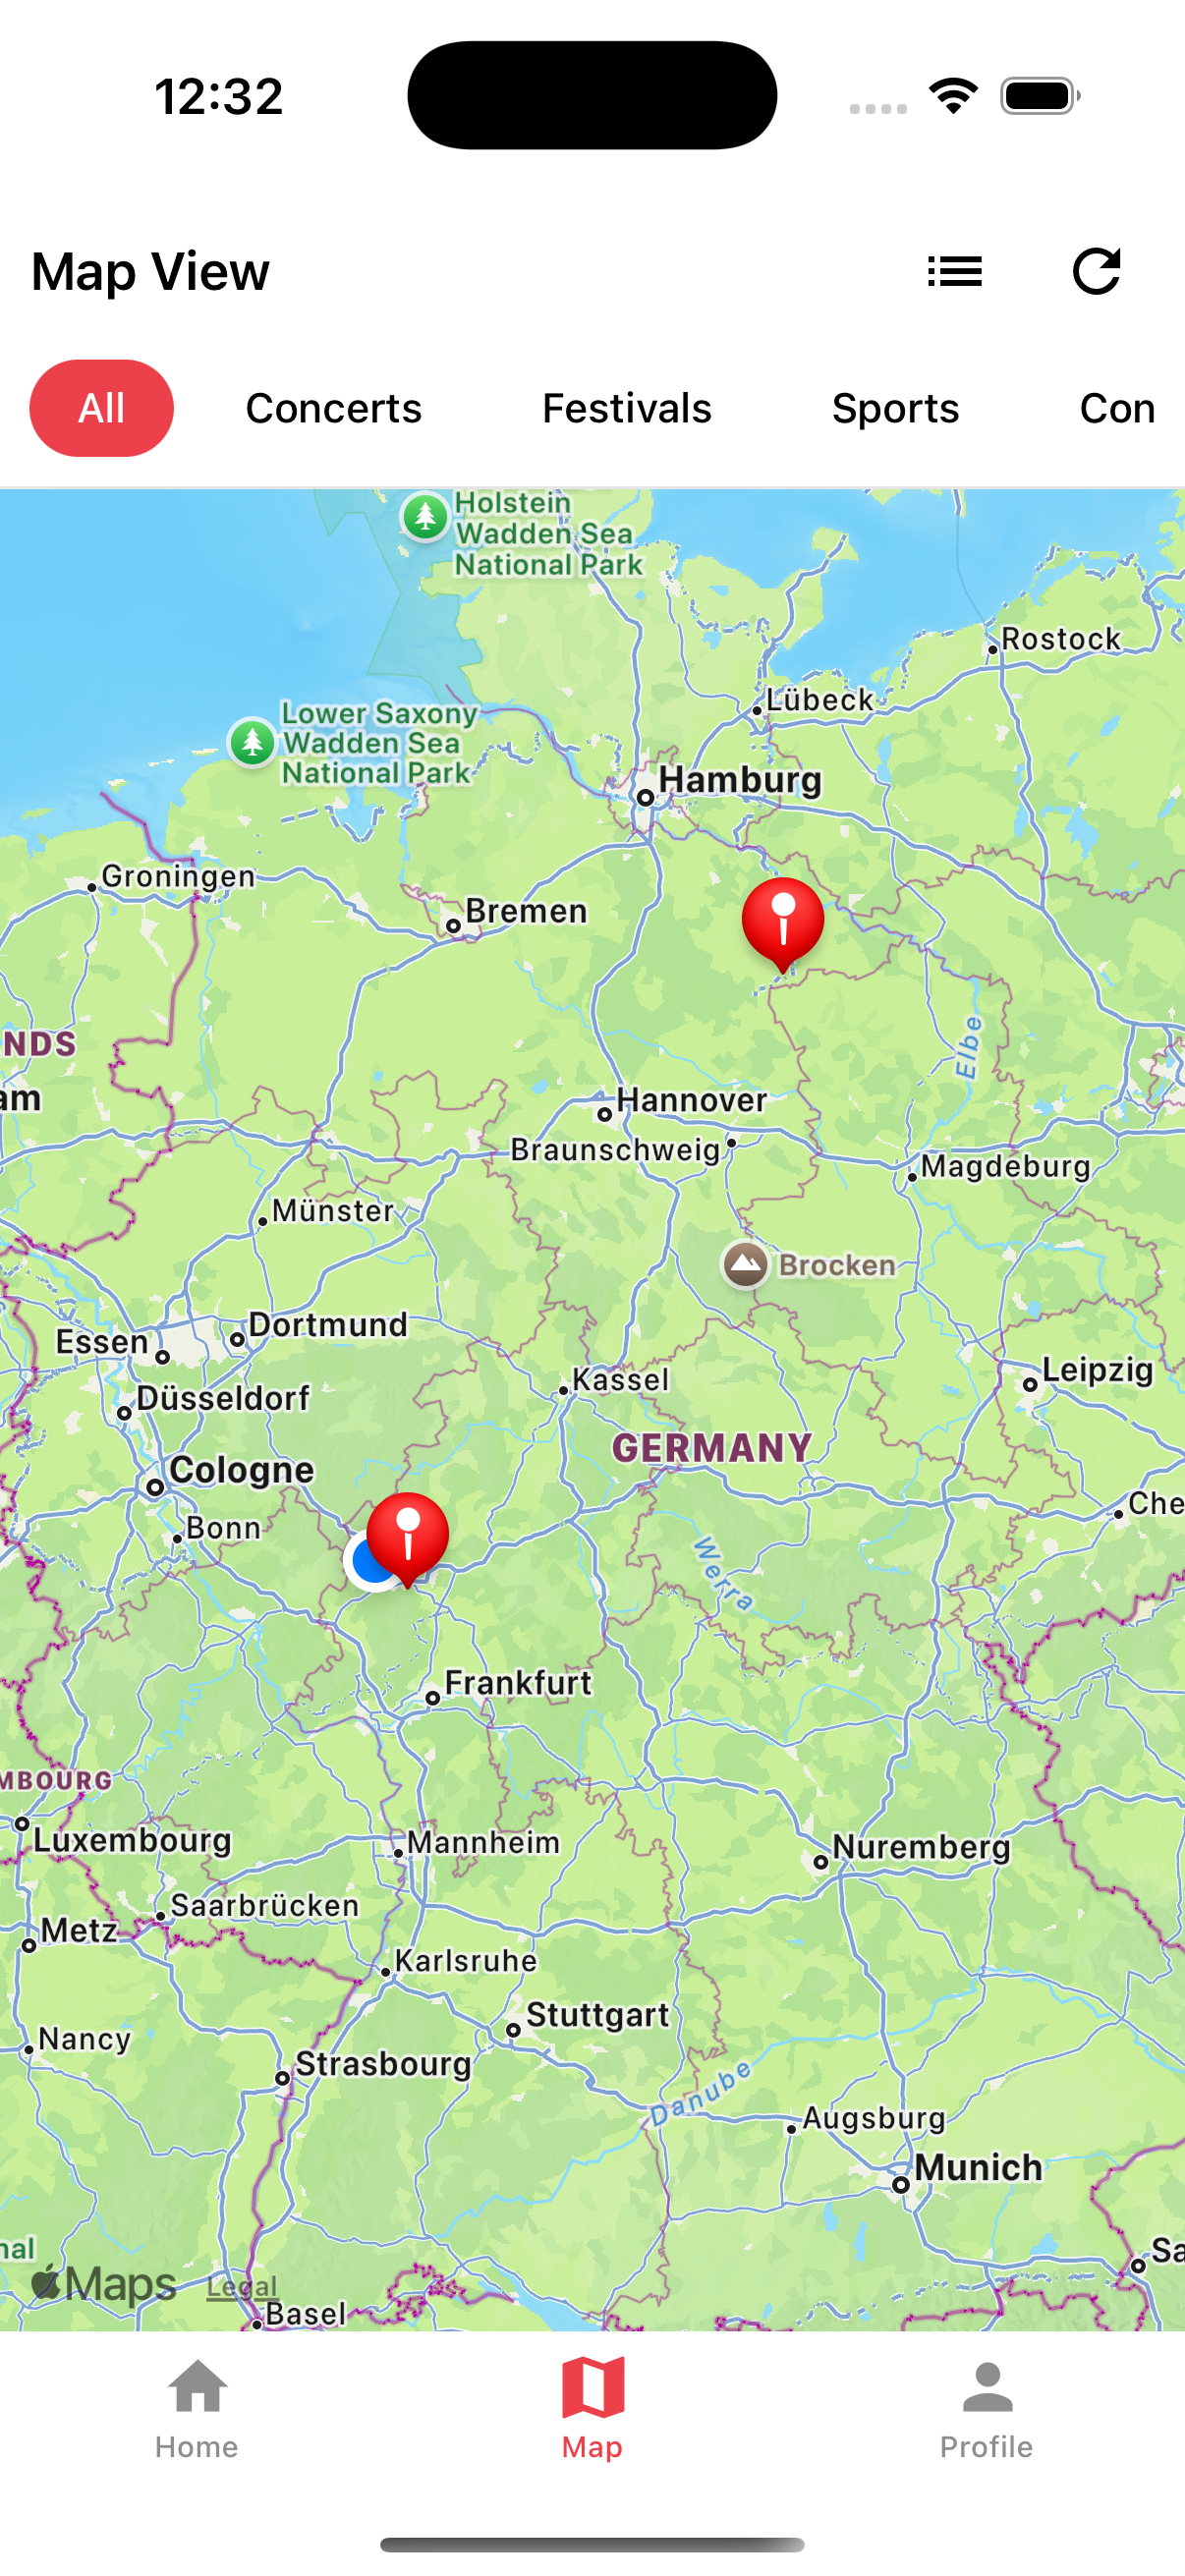
\includegraphics[width=0.98\textwidth]{images/cursor_screenshots/final-mapscreen-cursor-3.png}
      \end{minipage}
      \hfill
      \begin{minipage}{0.48\textwidth}
            \centering
            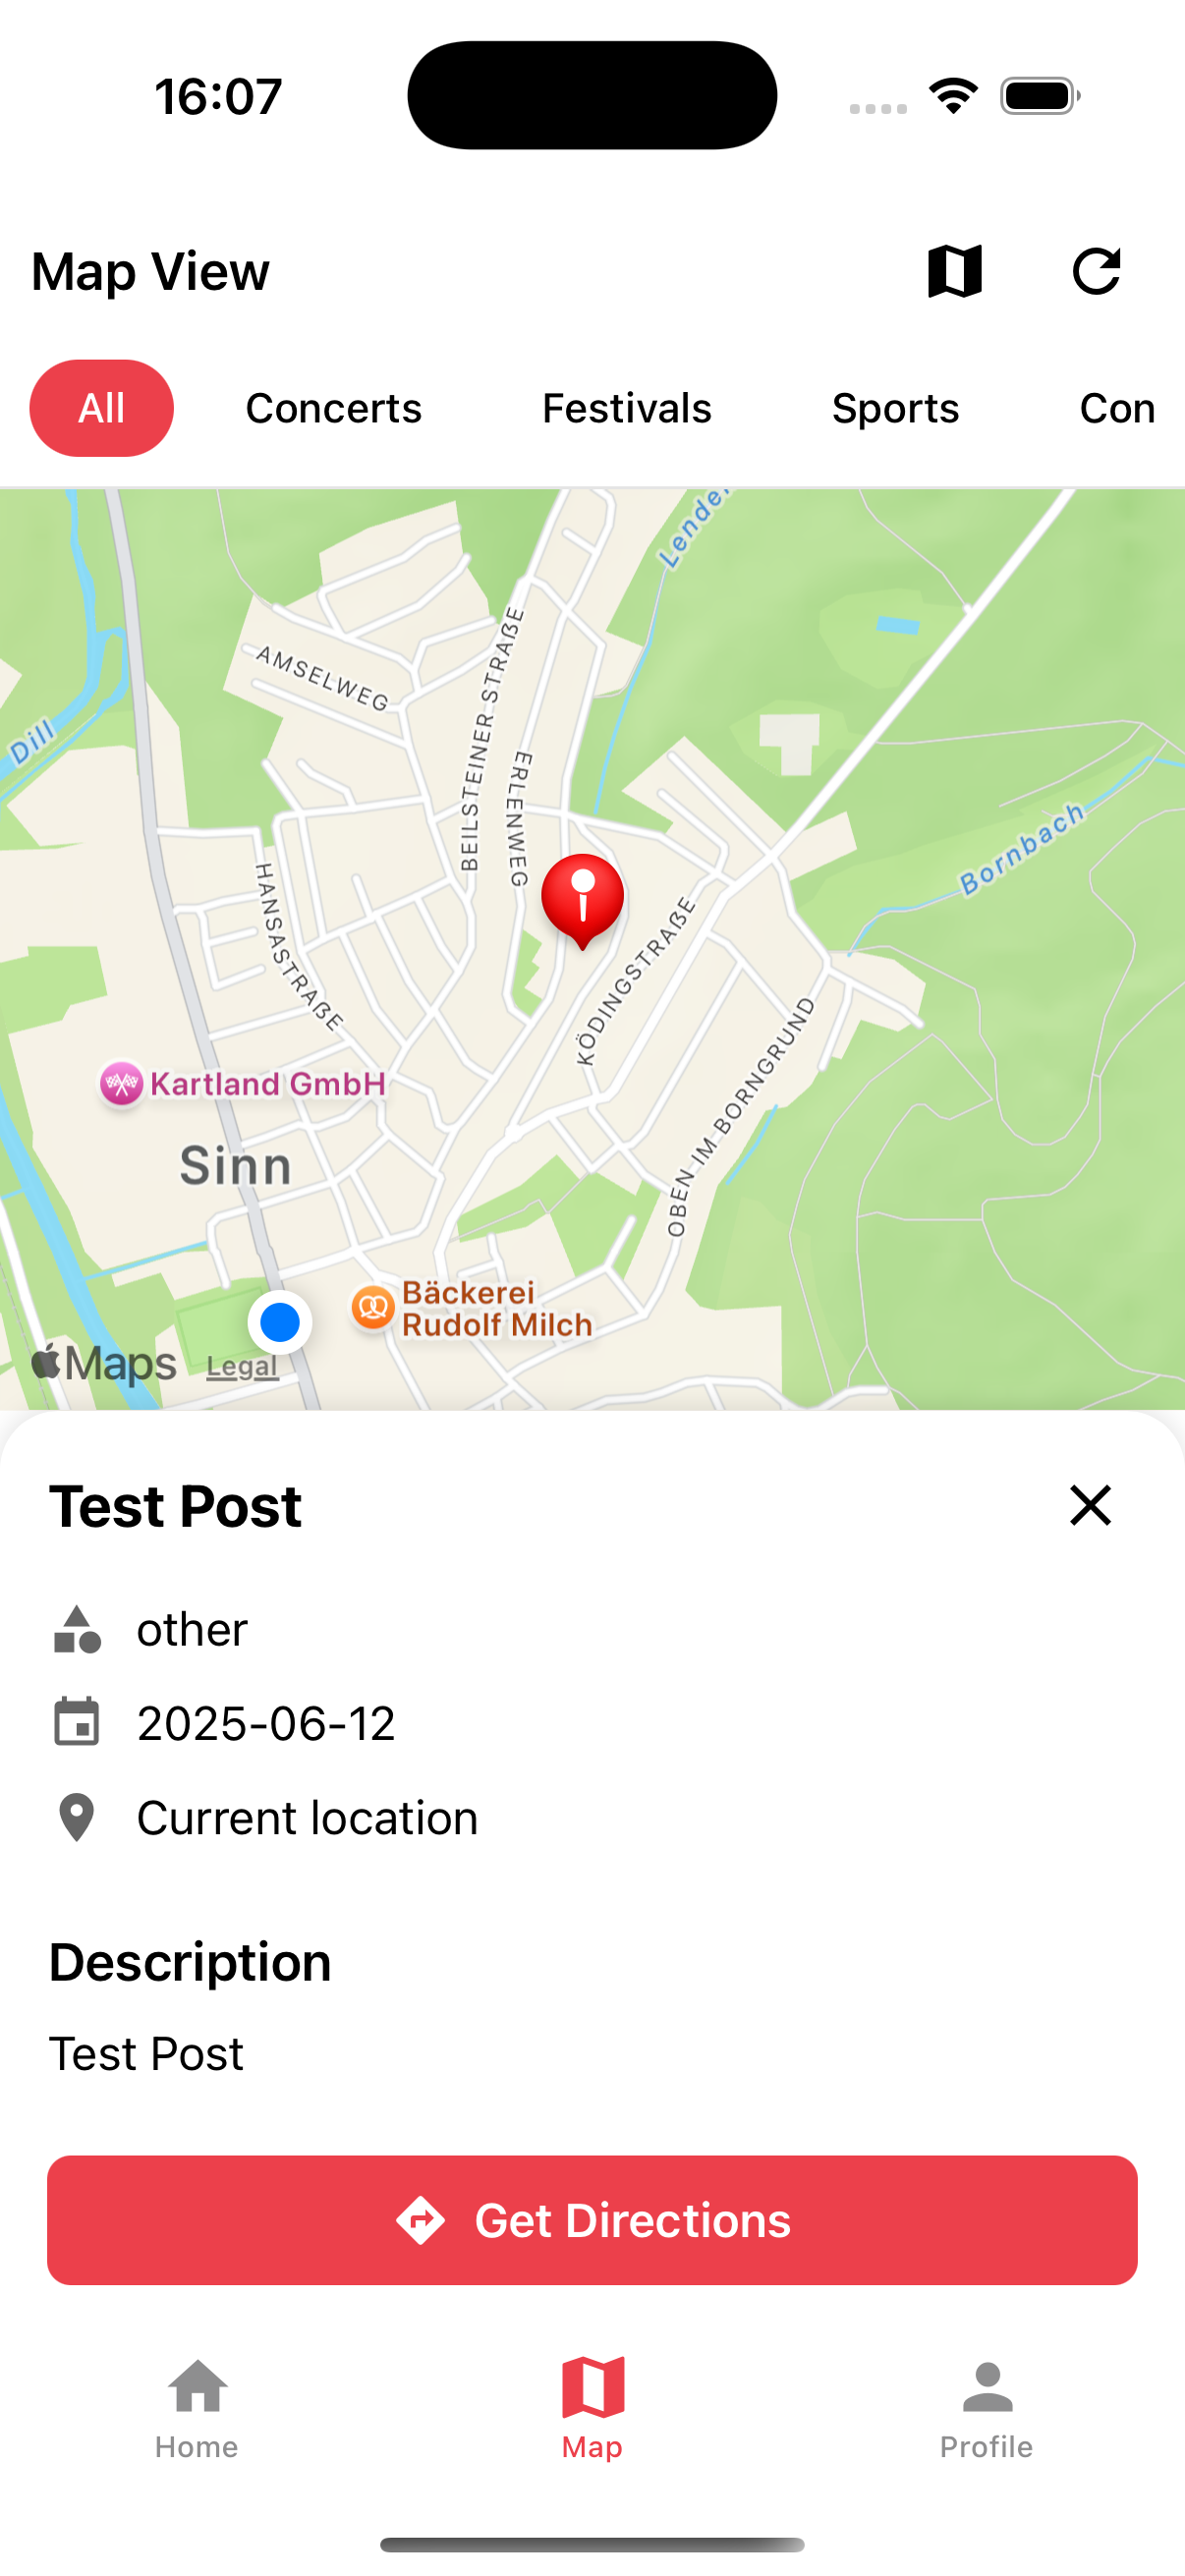
\includegraphics[width=0.98\textwidth]{images/cursor_screenshots/final-mapscreen-cursor-2.png}
      \end{minipage}
      \caption{MapScreen in der finalen Implementierung mit Cursor – zwei verschiedene Zustände/Ansichten. \textit{Cursor-Demo}}
      \label{fig:cursor-finalpair}
\end{figure}

\textbf{Herausforderungen und Learnings:}
\begin{itemize}
      \item Kompatibilitätsprobleme zwischen \texttt{react-native-maps} und Expo führten zu
            Fehlern, die erst nach mehreren Iterationen und Prompts gelöst wurden.
      \item Cursor wechselte in einem Schritt das Map-Framework, was manuell rückgängig
            gemacht wurde.
      \item Die Behandlung von Kategorie-Filtern führte zu denselben Herausforderungen wie
            bei Copilot, wurde aber durch gezielte Korrekturen gelöst.
      \item Cursor reagierte auf TypeErrors konsistent und ergänzte die notwendigen
            Anpassungen selbstständig.
\end{itemize}

\textbf{Reflexion:}
\begin{itemize}
      \item Die Entwicklung mit Cursor verlief insgesamt sehr zügig, da
            Kontextinformationen effektiv genutzt wurden.
      \item Die Vorschläge für komplexe UI- und Layout-Probleme waren oft präziser als bei
            Copilot.
      \item Der dialogische Ablauf mit Feedback-Loops war für iteratives Refactoring
            besonders hilfreich.
      \item Bei seltenen KI-Fehlinterpretationen war weiterhin manuelle Kontrolle nötig.
\end{itemize}

\textbf{Fazit:}
Cursor bewährt sich vor allem durch die Fähigkeit, Kontext (Screenshots, Code, Fehlermeldungen) aktiv in die Entwicklung einzubinden. Im Vergleich zu Copilot zeigte Cursor bei Debugging, Package-Fehlern und iterativen Verbesserungen eine hohe Präzision und Transparenz.

\subsection{Demonstration mit Bolt}

\subsubsection{Setup und Vorgehen}
Für die Entwicklung des Map-Screens wurde das KI-Assistenztool
\textbf{Bolt.new} eingesetzt. Bolt ermöglichte dabei den direkten Zugriff auf
das bestehende \texttt{Locals}-GitHub-Repository und bot eine integrierte
Umgebung für Prompt Chaining und Live-Code-Editing. Die identische
Aufgabenstellung wurde zu Beginn eingebracht (\emph{siehe
      Abschnitt~\ref{sec:prompt-setup}}).

\begin{figure}[htbp]
      \centering
      \vspace{1em}
      \begin{minipage}{0.48\textwidth}
            \centering
            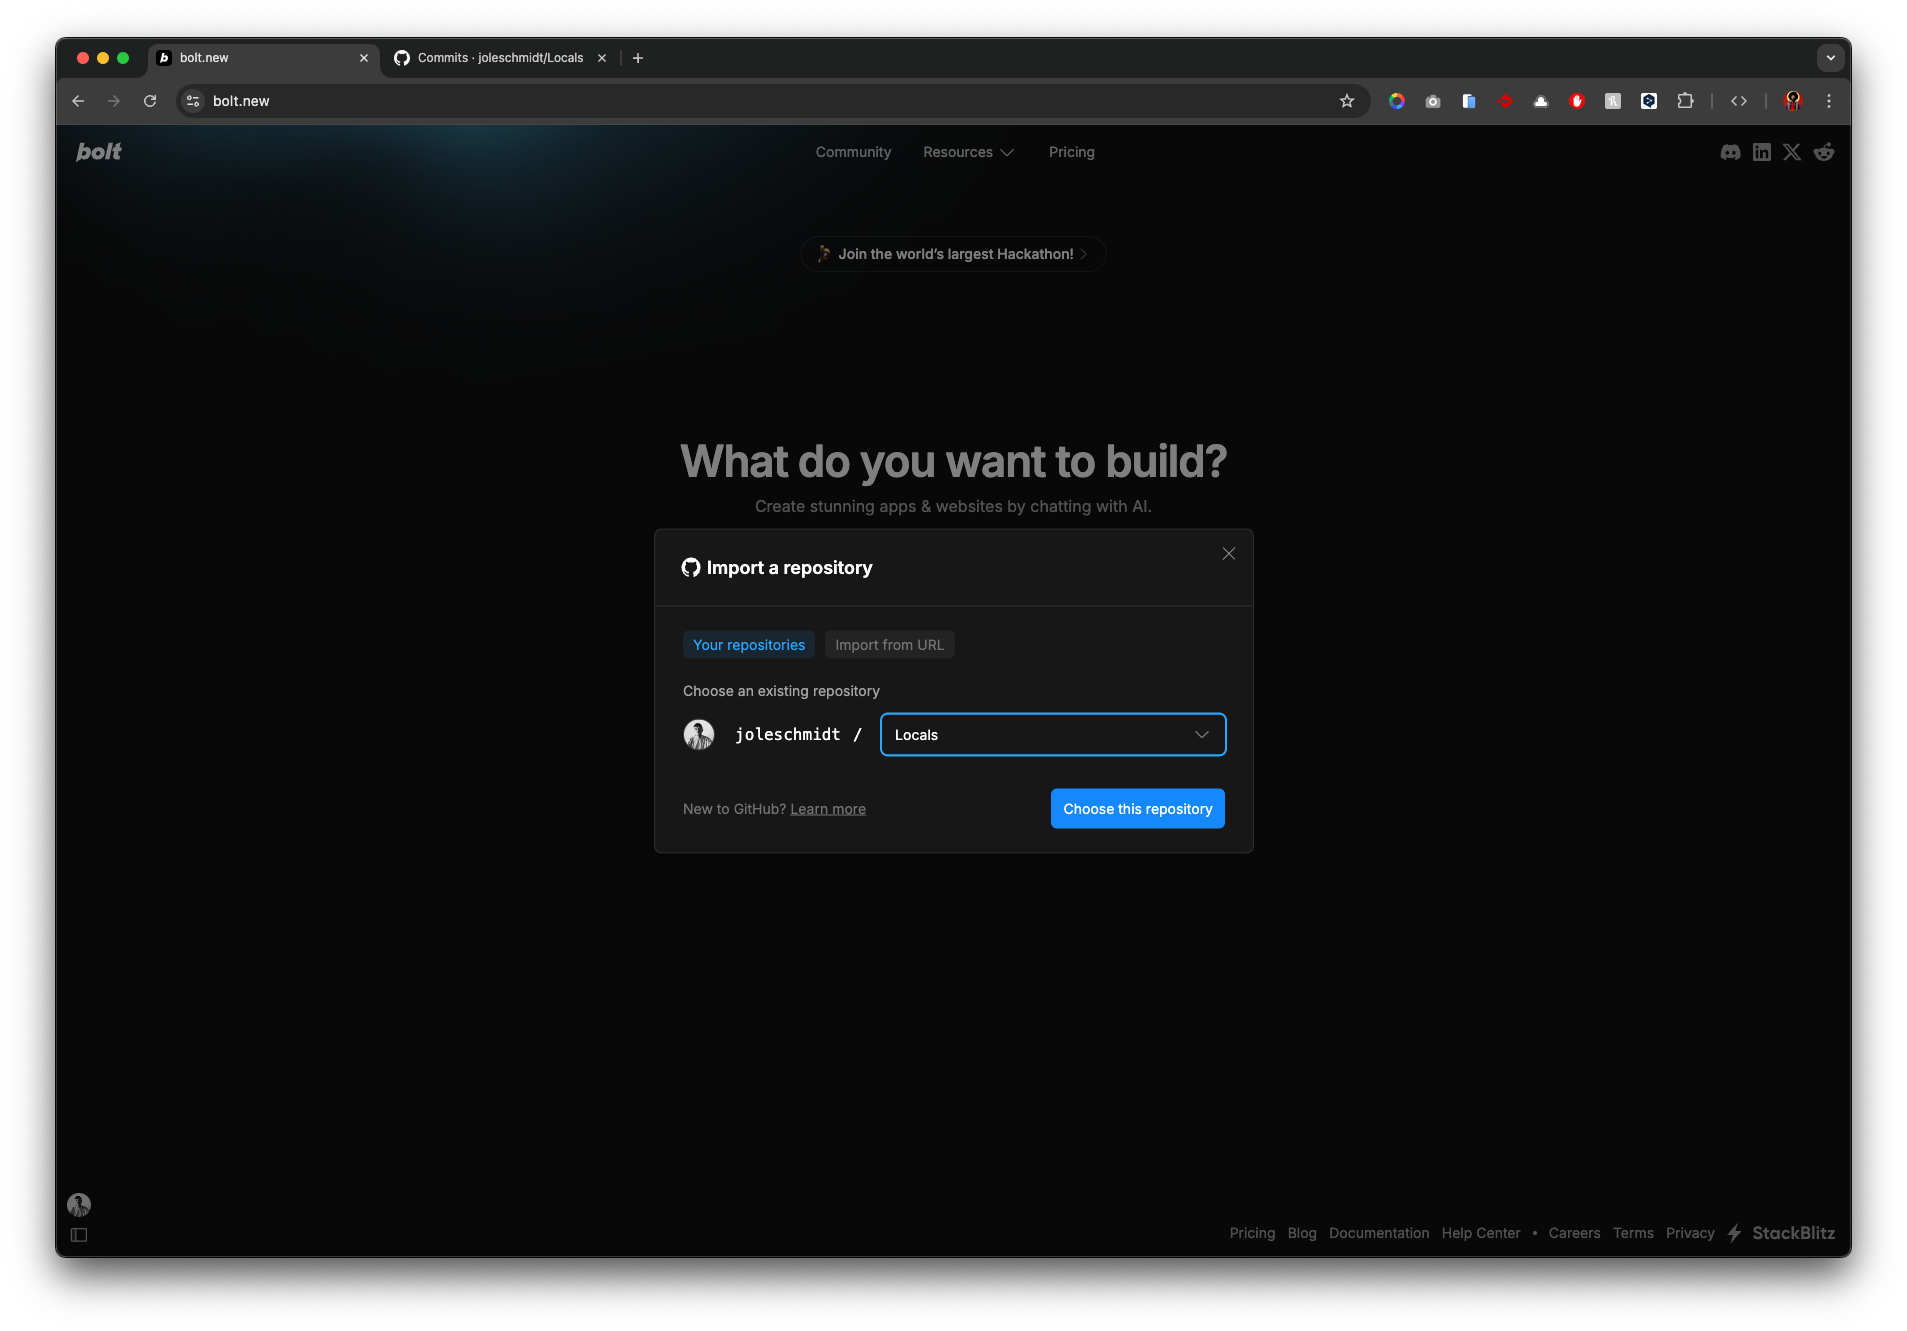
\includegraphics[width=0.98\textwidth]{images/bolt_screenshots/startseite-what-do-you-wanna-build-mit-github-branch.png}
      \end{minipage}
      \hfill
      \begin{minipage}{0.48\textwidth}
            \centering
            \includegraphics[width=0.98\textwidth]{images/bolt_screenshots/ der server funktioniert und bolt installiert die restlichen dependencies. scheinbar wird react-native-web benötigt um die laufende app zu sehen.png}
      \end{minipage}
      \caption{Links: Start mit Bolt.new und Auswahl des Locals-Repos. Rechts: Bolt erkennt fehlende Dependencies und installiert diese selbstständig. \textit{bolt-Demo}}
      \label{fig:bolt-setup}
\end{figure}

Zu Beginn wurden Screenshots des aktuellen App-Zustands sowie zentrale
Komponenten als Kontext bereitgestellt.

\subsubsection{Schrittweise Umsetzung und Reflexion}
Die Besonderheit bei Bolt lag im engen Zusammenspiel mit GitHub, den
automatisch ausführbaren Terminalbefehlen sowie der Möglichkeit, nativ Pakete
zu installieren und Fehler im laufenden Betrieb zu beheben.

\begin{figure}[htbp]
      \centering
      \vspace{1em}
      \begin{minipage}{0.48\textwidth}
            \centering
            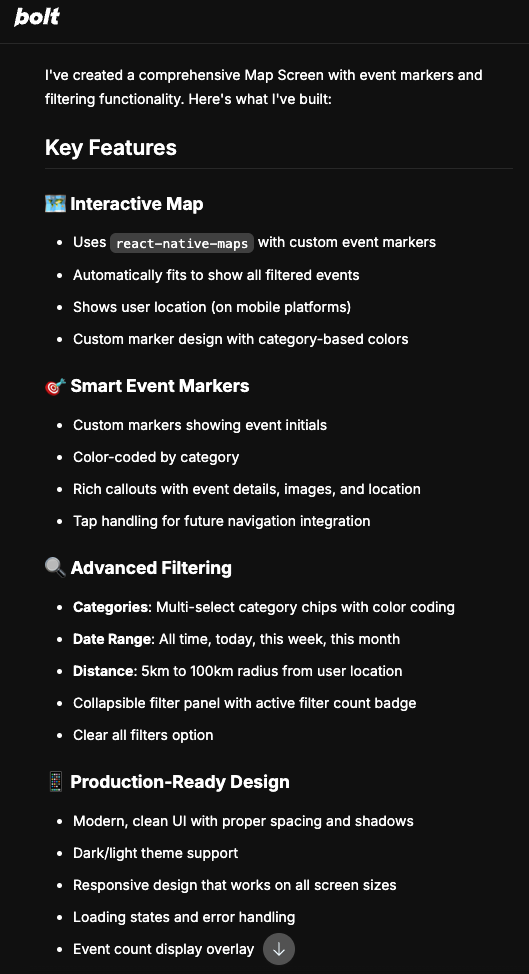
\includegraphics[width=0.98\textwidth]{images/bolt_screenshots/eingabe des prompts-rueckmeldung von bolt-1.png}
      \end{minipage}
      \hfill
      \begin{minipage}{0.48\textwidth}
            \centering
            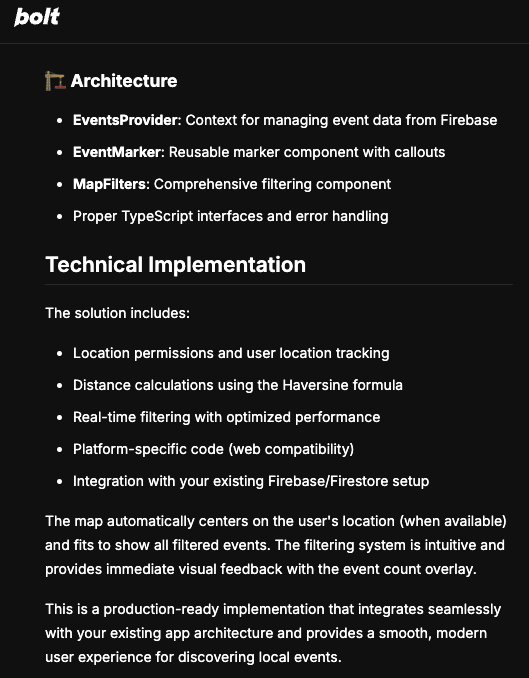
\includegraphics[width=0.98\textwidth]{images/bolt_screenshots/eingabe des prompts-rueckmeldung von bolt-2.png.png}
      \end{minipage}
      \caption{Bolt reagiert interaktiv auf Prompts, führt Terminalbefehle aus und gibt strukturiertes Feedback im Interface. \textit{bolt-Demo}}
      \label{fig:bolt-prompts}
\end{figure}

\textbf{Ablauf:}
\begin{enumerate}
      \item \textbf{Repository-Anbindung und Initialisierung:} Über die GitHub-Integration wurde direkt auf das Locals-Repo zugegriffen, ein neuer Branch erstellt und Bolt konnte sämtliche Projektdaten einsehen.
      \item \textbf{Prompt Chaining und Kontextgabe:} Für jede Aufgabe wurden Prompts mit Screenshots und Codeausschnitten ergänzt, etwa zur Installation fehlender Abhängigkeiten wie \texttt{react-native-web}.
      \item \textbf{Automatisiertes Debugging:} Terminalbefehle wie \texttt{npm run dev} wurden selbständig ausgeführt, Fehler wie inkompatible Packages oder fehlende Dependencies eigenständig erkannt und (teilweise) gelöst.
      \item \textbf{Feature-Integration:} Bolt erstellte zentrale Komponenten (\texttt{EventsProvider}, \texttt{EventMarker}, \texttt{MapFilters}) und aktualisierte \texttt{map.tsx} und \texttt{map.web.tsx} für mobile und Web.
      \item \textbf{Multi-Plattform-Support:} Bei Problemen mit \texttt{react-native-maps} auf Web wurde automatisch auf \texttt{react-google-maps} gewechselt und eine alternative Map-Implementierung für Web ergänzt.
      \item \textbf{Fehler-Handling und Limits:} Bei aufwendigen Operationen wurde das Tageslimit des kostenlosen Bolt-Plans schnell erreicht, was ein Upgrade auf Pro erforderte.
\end{enumerate}

\begin{figure}[htbp]
      \centering
      \vspace{1em}
      \begin{minipage}{0.48\textwidth}
            \centering
            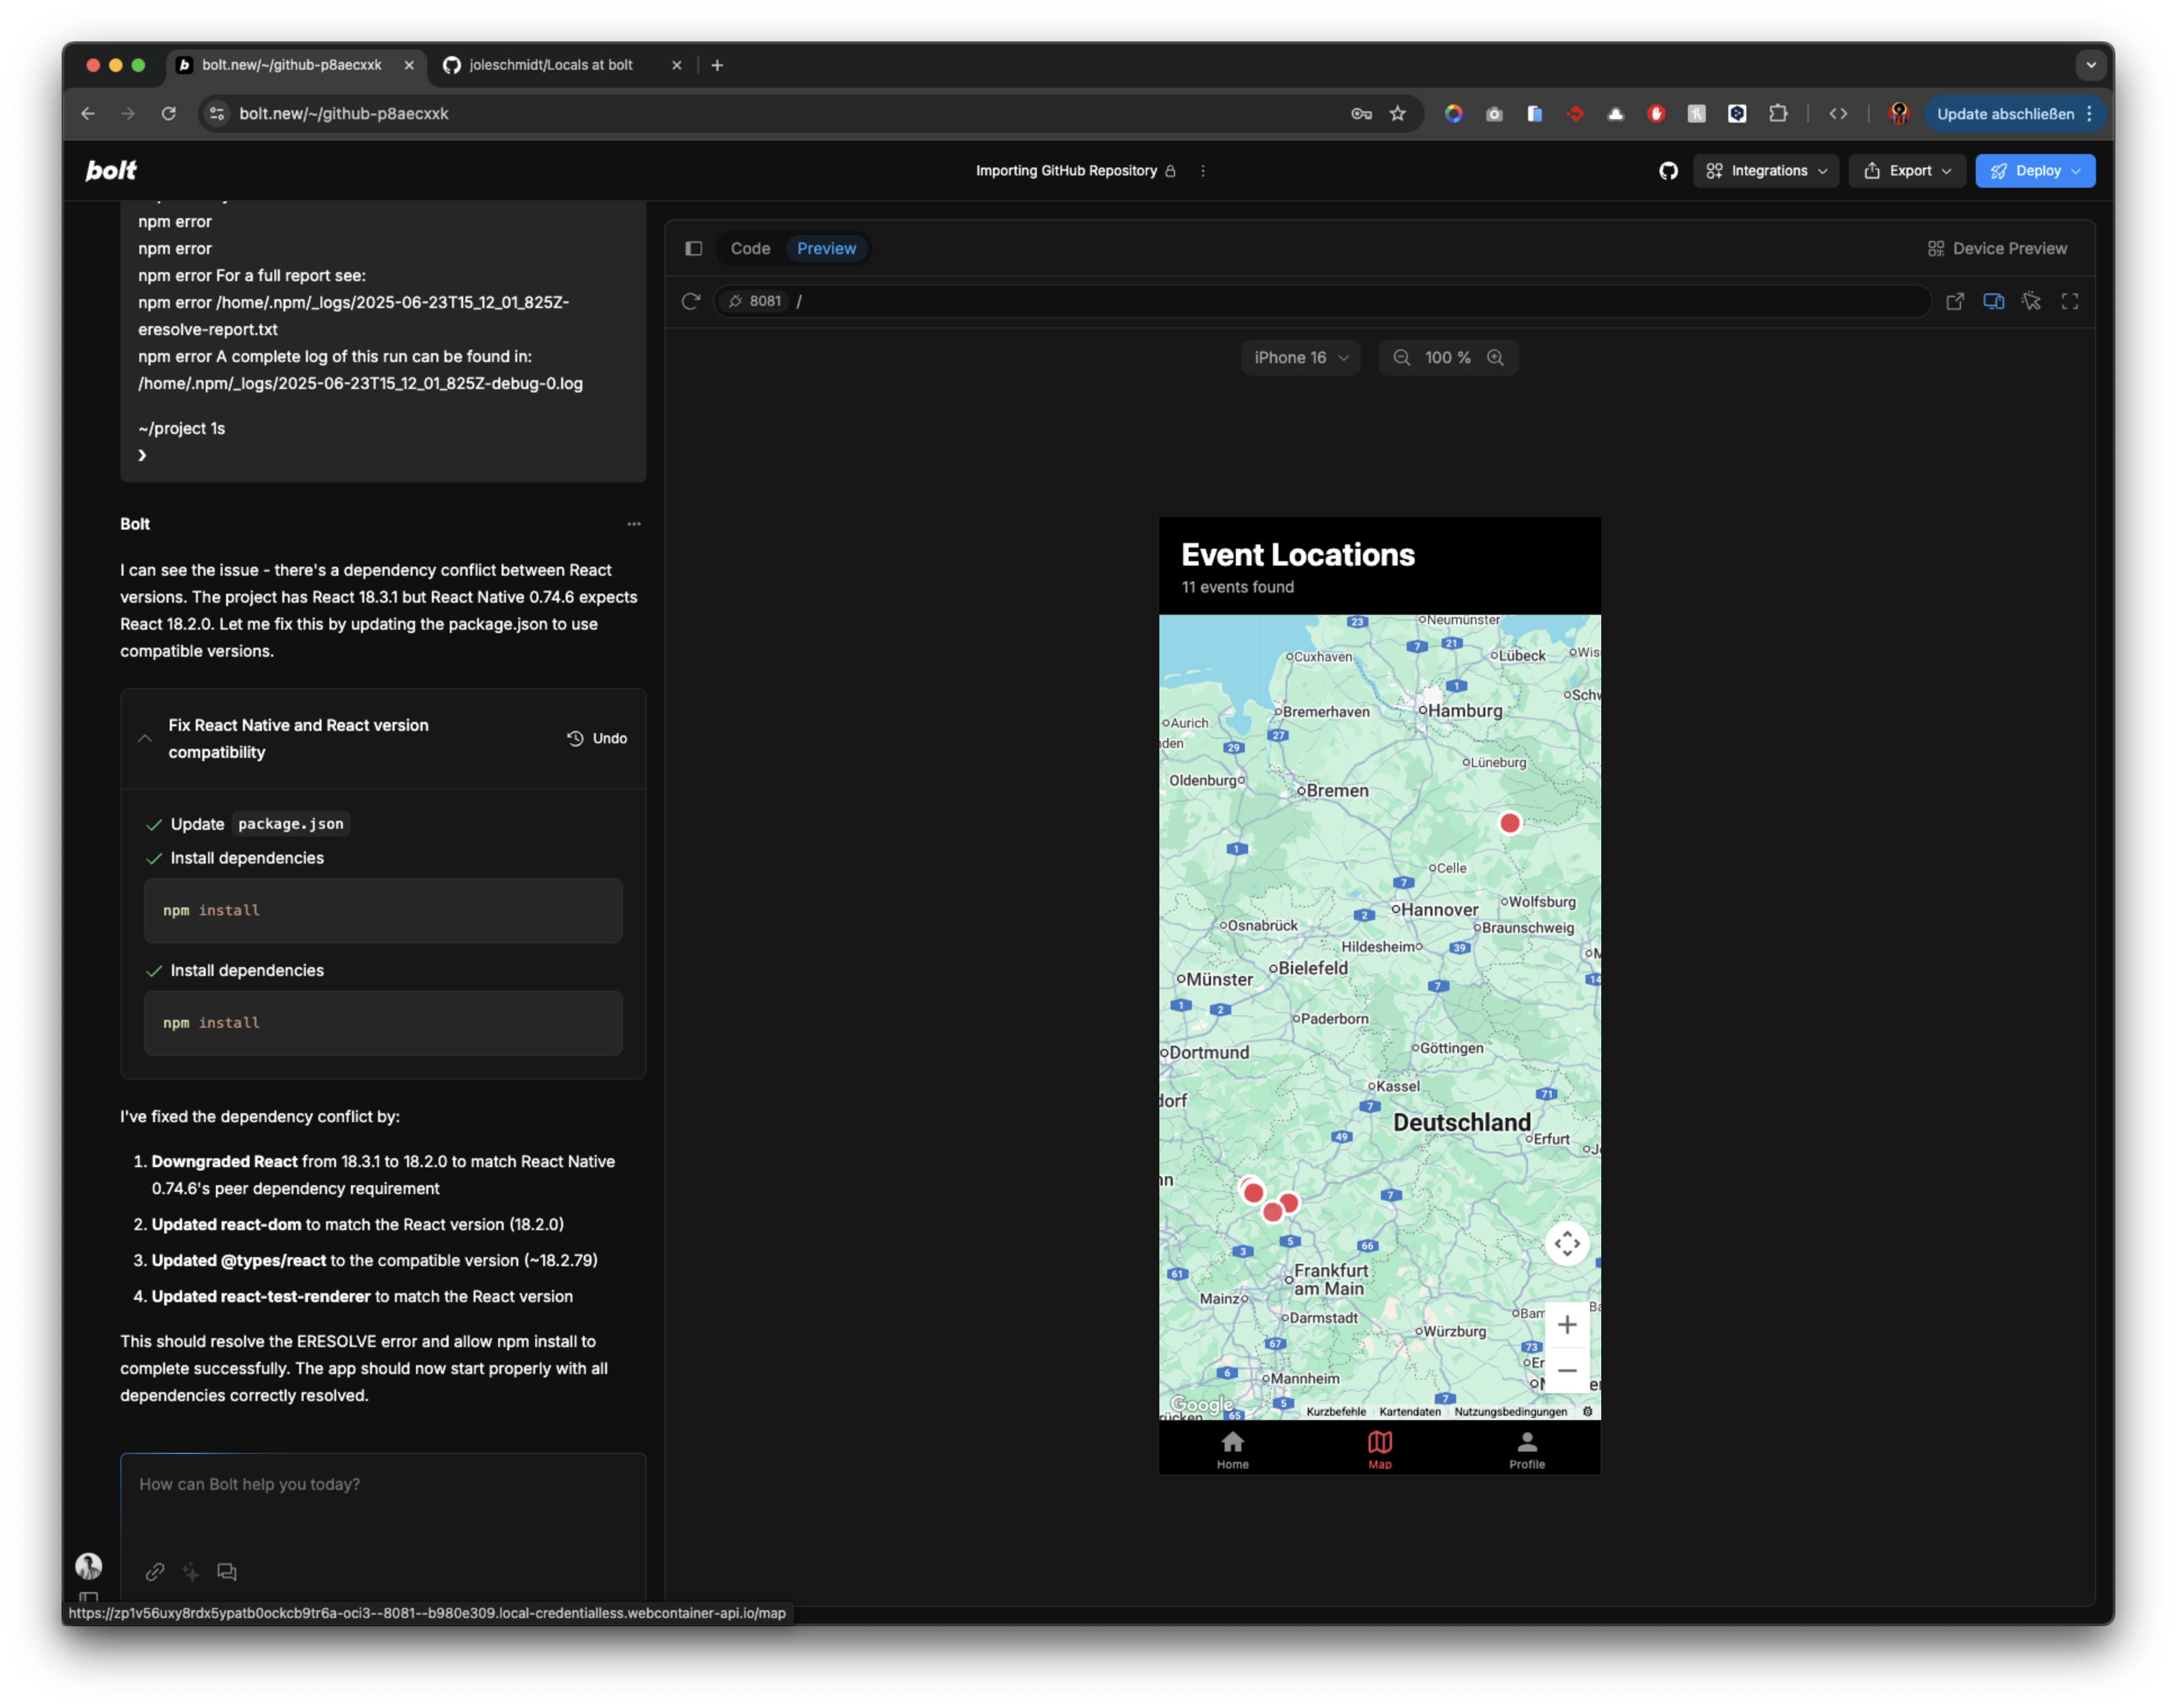
\includegraphics[width=0.98\textwidth]{images/bolt_screenshots/funktionierender map screen.png}
      \end{minipage}
      \hfill
      \begin{minipage}{0.48\textwidth}
            \centering
            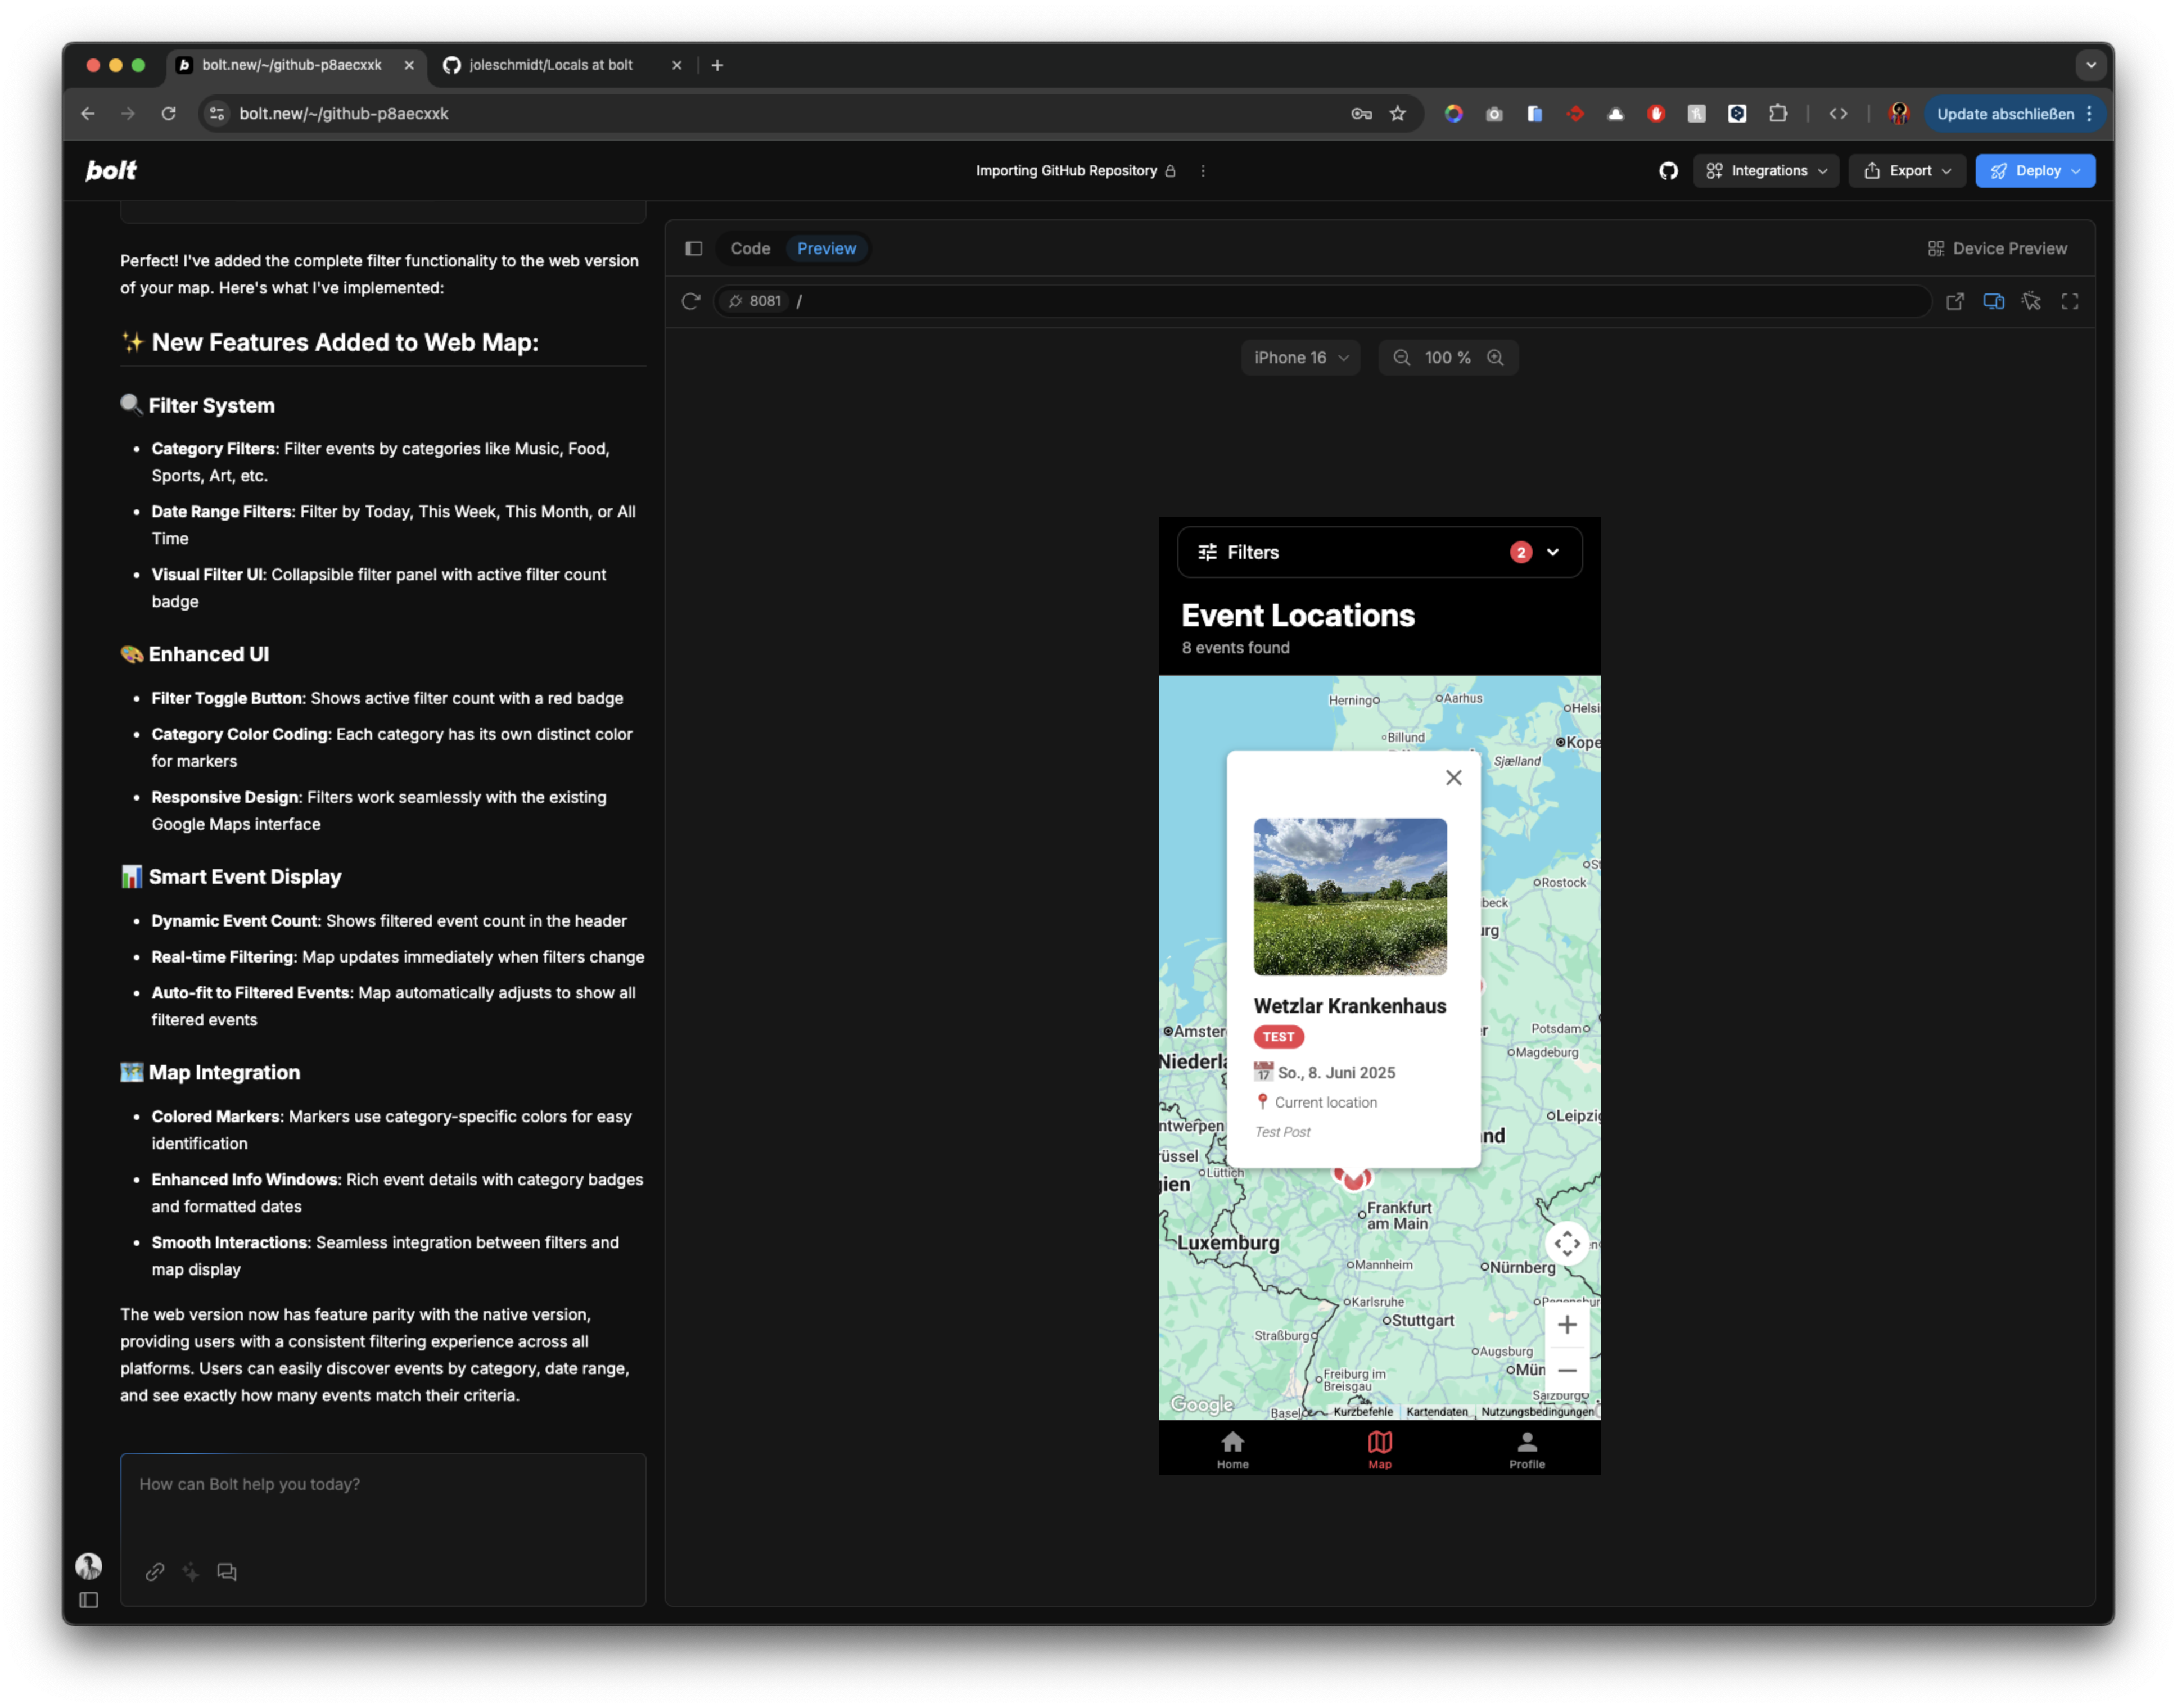
\includegraphics[width=0.98\textwidth]{images/bolt_screenshots/funktionierender map screen + callout & filter angewendet.png}
      \end{minipage}
      \caption{Finale Web-Umsetzung: Interaktiver MapScreen mit Event-Details, Filteroptionen und Callouts. \textit{bolt-Demo}}
      \label{fig:bolt-final}
\end{figure}

\textbf{Herausforderungen und Learnings:}
\begin{itemize}
      \item Bolt war in der Lage, das Setup und viele Standard-Probleme selbständig zu
            lösen und bot zudem intuitive Web-Deployments.
      \item Die Filterlogik, insbesondere der Kategorie-Filter, wurde als einziges KI-Tool
            auf Anhieb korrekt umgesetzt.
      \item Komplexere Fehler (z.\,B. inkompatible native Packages bei mobilen Builds,
            Firebase-Probleme auf iOS) konnten von Bolt erkannt, aber nicht nachhaltig
            gelöst werden.
      \item Die parallele Unterstützung für mobile und Web führte zu umfangreichen
            Anpassungen und wiederkehrenden Fehlern, insbesondere bei der Koordination von
            Dependencies.
      \item Das Token- und Tageslimit der Free-Version wurde durch wiederholte Fehlersuche
            und Build-Versuche schnell ausgereizt.
\end{itemize}

\textbf{Reflexion:}
\begin{itemize}
      \item Bolt eignet sich besonders gut für grüne Wiese-Projekte, kleine neue Repos oder
            als Unterstützung bei der Initialisierung und Standardisierung. Die direkte
            GitHub-, Stripe- und Supabase-Integration sowie das Web-Deployment sind hier
            besonders hilfreich.
      \item Bei größeren, bereits bestehenden Projekten stößt Bolt aktuell jedoch an seine
            Grenzen: Zwar konnte ein funktionierender Map-Screen für das Web erstellt
            werden, für mobile Builds blieben die Fehler jedoch bestehen.
      \item Die Fehlererkennung und automatische Problemlösung war überzeugend, für
            nicht-triviale Projekte bleibt jedoch manuelle Nacharbeit und kritisches Review
            unerlässlich.
      \item Die Web-App ist insgesamt modern und intuitiv gestaltet.
\end{itemize}

\textbf{Fazit:}
Bolt kann den Entwicklungsprozess – besonders in neuen Projekten – signifikant beschleunigen und standardisieren. Bei komplexeren Setups oder plattformübergreifenden Anforderungen treten jedoch noch Limitierungen auf, die nicht ohne weiteres automatisch gelöst werden können.

% ----------- Vergleich und Bewertung
\subsection{Vergleich und Bewertung der eingesetzten KI-Tools}

Nach der Durchführung der Demonstrationen mit Copilot, Cursor und Bolt werden
Unterschiede und Gemeinsamkeiten hinsichtlich Funktionalität, Effizienz,
Entwicklererlebnis und Ergebnisqualität sichtbar.

\subsubsection{Direkter Vergleich}

\begin{itemize}
      \item \textbf{Copilot} überzeugt besonders bei Standardaufgaben und bewährten Patterns in der Codegenerierung. Die Effizienzsteigerung bei Routinearbeiten ist erheblich, bei komplexeren Anforderungen bleibt jedoch manuelle Nacharbeit nötig.
      \item \textbf{Cursor} ermöglicht durch aktiven Kontextbezug (Screenshots, Code, Fehlermeldungen) und dialogisches Prompt Chaining eine zielgerichtete und schnelle Entwicklung. Die Fehlerdiagnose und Lösungsvorschläge sind präziser als bei Copilot, bei Spezialfällen ist aber weiterhin aktive Begleitung nötig.
      \item \textbf{Bolt} punktet mit umfassender Plattformintegration (GitHub, Web, App Store) und der Möglichkeit, Projekte direkt aus der Cloud-IDE zu initialisieren und zu deployen. Besonders im Web-Kontext zeigt Bolt große Stärken, stößt jedoch bei der mobilen Entwicklung und beim Refactoring bestehender Projekte an Grenzen.
\end{itemize}

Die Ergebnisse dieser Demonstration stehen im Einklang mit aktuellen Studien,
die Effizienzgewinne und Qualitätsverbesserungen durch generative KI-Tools
nachweisen. Coutinho et~al.~\cite{coutinho_role_2024} berichten von deutlicher
Zeitersparnis bei Standardaufgaben, während Braun~\cite{braun_ki_2024} und
Sulabh~\cite{s_future_2024} auf die weiterhin bestehende Notwendigkeit
manueller Kontrolle und Überprüfung hinweisen. Schmitt
et~al.~\cite{schmitt_generative_2024} betonen zudem, dass KI-Tools auch soziale
und identitätsbezogene Veränderungen im Entwickleralltag nach sich ziehen.

\subsubsection{Lessons Learned und Best Practices}

Die praktische Evaluation zeigt: Generative KI-Tools sind eine wertvolle
Unterstützung im Entwicklungsprozess und führen – bei richtiger Anwendung – zu
Effizienzgewinnen, höherer Codequalität und einer Steigerung des
Entwicklererlebnisses. Wesentliche Empfehlungen lassen sich ableiten:

\begin{itemize}
      \item \textbf{Präzise Prompts sind essenziell:} Je konkreter und kontextreicher die Anweisungen, desto passgenauer das Ergebnis.
      \item \textbf{Manuelle Kontrolle bleibt notwendig:} Trotz hoher Automatisierung ist die Überprüfung aller KI-generierten Änderungen unerlässlich.
      \item \textbf{Kontextnutzung und Feedback-Loops:} Tools wie Cursor, die Kontextinformationen aktiv verarbeiten, bieten klare Vorteile bei komplexeren Aufgaben.
      \item \textbf{Tool-Auswahl nach Projekttyp:} Für neue Projekte oder Prototypen eignen sich Tools wie Bolt, für laufende Projekte Copilot (Routine) oder Cursor (komplexere, dialogische Abläufe).
      \item \textbf{Plattformkompatibilität beachten:} Verschiedene Plattformen erfordern oft eigene Anpassungen – dies wird von den Tools unterschiedlich gut unterstützt.
\end{itemize}

\subsubsection{Qualitative Bewertung: Zeiteffizienz, Codequalität und Wartbarkeit}

Die Analyse zeigt differenzierte Ergebnisse:
\begin{itemize}
      \item \textbf{Copilot:} Spürbare Zeitersparnis bei Standardaufgaben, solide Codequalität bei Routinetätigkeiten, Nacharbeit nötig bei individueller Logik.
      \item \textbf{Cursor:} Schnelles Debugging, zielgerichtete Entwicklung dank Kontextintegration, hohe Zeiteffizienz und verbesserte Wartbarkeit.
      \item \textbf{Bolt:} Große Stärken bei Projektinitialisierung und Multi-Plattform-Support, Zeiteinsparung besonders im Setup, aber Kompatibilitätsprobleme im laufenden Betrieb.
\end{itemize}

\subsection{Zwischenfazit}

Die praktische Demonstration liefert zentrale Erkenntnisse: Generative KI-Tools
ermöglichen signifikante Effizienzsteigerungen bei Routineaufgaben und bieten
Potenziale für höhere Codequalität und Wartbarkeit. Gleichzeitig treten
Herausforderungen bei Fehlerbehebung, Tool-Integration und
plattformübergreifender Entwicklung auf. Diese Erfahrungen bilden die Grundlage
für die systematische Bewertung der Chancen und Risiken generativer KI in der
Softwareentwicklung in den folgenden Kapiteln.

Aktuelle Forschungsergebnisse bestätigen diese Beobachtungen: Aspekte wie
Barrierefreiheit und Usability sollten laut Flores-Saviaga
et~al.~\cite{flores-saviaga_impact_2025} künftig stärker berücksichtigt werden.
Geyer et~al.~\cite{geyer_case_2025} zeigen, dass die Integration generativer
KI-Tools auch positive Effekte auf Teamarbeit und Qualitätssicherung in agilen
Entwicklungsprojekten haben kann.
